\documentclass[7Sketches]{subfiles}
\begin{document}

\setcounter{chapter}{1}%Just finished 1.
%------------ Chapter ------------%
\chapter[Resources: monoidal preorders and enrichment]{Resource theories:\\Monoidal preorders and enrichment} %
\label{chap.resource_theory}

%\settocdepth{subsubsection}
%\clearpage
%\tableofcontents*

%-------- Section --------%
\section{Getting from $a$ to $b$}%
\index{resource!theory|(}

You can't make an omelette without breaking an egg. To obtain the things we want requires resources, and the process of transforming what we have into what we want is often an intricate one. In this chapter, we will discuss how monoidal preorders can help us think about this matter.

Consider the following three questions you might ask yourself:
\begin{itemize}
	\item Given what I have, is it \emph{possible} to get what I want?
	\item Given what I have, what is the \emph{minimum cost} to get what I want?
	\item Given what I have, what is the \emph{set of ways} to get what I want?
\end{itemize}
These questions are about resources---those you have and those you want---but perhaps more importantly, they are about moving from have to want: possibility of, cost of, and ways to.

Such questions come up not only in our lives, but also in science and industry. In chemistry, one asks whether a certain set of compounds can be transformed into another set, how much energy such a reaction will require, or what methods exist for making it happen. In manufacturing, one asks similar questions.
%
\index{chemistry}
%
\index{manufacturing}

From an external point of view, both a chemist and an industrial firm might be regarded as store-houses of information on the above subjects. The chemist knows which compounds she can make given other ones, and how to do so; the firm has stored knowledge of the same sort. The research work of the chemist and the firm is to use what they know in order to derive---or discover---new knowledge.

This is roughly the first goal of this chapter: to discuss a formalism for expressing recipes---methods for transforming one set of resources into another---and for deriving new recipes from old. The idea here is not complicated, neither in life nor in our mathematical formalism. The value added then is to simply see how it works, so we can build on it within the book, and so others can build on it in their own work.%
\index{recipes}

We briefly discuss the categorical approach to this idea---namely that of
\emph{monoidal preorders}---for building new recipes from old. The following
\emph{wiring diagram} shows, assuming one knows how to implement each of the
interior boxes, how to implement the preparation of a lemon meringue
pie:%
\index{pie!lemon meringue}%
\index{wiring diagram}
\begin{equation}%
\label{eqn.how_to_bake_pie}
\begin{tikzpicture}[oriented WD, align=center, bbx=1.2cm, bby=2ex]
	\node[bb={4}{1}, bb min width=.9in] (filling) {make\\lemon\\filling};
	\node[bb={2}{1}, bb min width=.9in, below=of filling] (meringue) {make\\meringue};
	\node at ($(filling.west)!.5!(meringue.west)$) (helper) {};
	\node[bb={1}{2}, left = of helper] (separate) {separate\\egg};
	\node[bb={2}{1}, above right = -2 and 1 of filling] (fill) {fill crust};
	\node[bb={2}{1}, below right = of fill] (finish) {add\\meringue};
	\node[bb={0}{0}, bb name=prepare lemon meringue pie, fit={(separate) (meringue) ($(fill.north)+(0,2)$) (finish)}] (pie) {};
%
\begin{scope}[font=\tiny]
	\draw (pie.west|-fill_in1) to node[pos=.25, above] {prepared crust} (fill_in1);
	\draw (pie.west|-filling_in1) to node[above] {lemon} (filling_in1);
	\draw (pie.west|-filling_in2) to node[above] {butter} (filling_in2);
	\draw (pie.west|-filling_in3) to node[above] {sugar} (filling_in3);
	\draw (pie.west|-separate_in1) to node[above] {egg} (separate_in1);
	\draw (pie.west|-meringue_in2) to node[above] {sugar} (meringue_in2);
	\draw (separate_out1) to node[above] {yolk} (filling_in4);
	\draw (separate_out2) to node[fill=white, inner sep=0.8pt] {white} (meringue_in1);
	\draw (filling_out1) to node[fill=white, inner sep=0.8pt] {lemon\\filling} (fill_in2);
	\draw (fill_out1) to node[fill=white, inner sep=0.8pt] {unbaked\\lemon pie} (finish_in1);
	\draw let \p1=(fill.east|-meringue_out1), \n1=\bbportlen in
		(meringue_out1) to node[above] {meringue} (\x1+\n1,\y1) to (finish_in2);
	\draw (finish_out1) to node[above] {unbaked\\pie} (finish_out1-|pie.east);
\end{scope}
\end{tikzpicture}
\end{equation}
The wires show resources: we start with prepared crust, lemon, butter, sugar, and egg resources, and we end up with an unbaked pie resource. We could take this whole method and combine it with others, e.g.\ baking the pie:
\[
\begin{tikzpicture}[oriented WD, align=center, bbx=1.2cm, bby=2ex]
	\node[bb port sep=.4, bb={6}{1}] (prepare) {prepare lemon meringue pie};
	\node[bb={2}{2}, below right=-1 and 2 of prepare] (bake) {bake pie};
	\node[bb={0}{0}, fit=(prepare) (bake), inner xsep=1.6cm] (outer) {};
	\foreach \i in {1,...,6}	\draw (outer.west|-prepare_in\i) -- (prepare_in\i);
	\begin{scope}[font=\scriptsize]
		\draw (outer.west|-bake_in2) to node[below] {oven} (bake_in2);
		\draw (prepare_out1) to node[above, align=center] {unbaked\\pie} (bake_in1);
		\draw (bake_out1) to node[above] {baked pie} (bake_out1-|outer.east);
		\draw (bake_out2) to node[below] {oven} (bake_out2-|outer.east);
	\end{scope}
\end{tikzpicture}
\]
In the above example we see that resources are not always consumed when they are used. For example, we use an oven to convert---or catalyze the transformation of---an unbaked pie into a baked pie, and we get the oven back after we are done. It's a nice feature of ovens! To use economic terms, the oven is a ``means of production'' for pies.

String diagrams are important mathematical objects that will come up repeatedly in this book. They were invented in the mathematical context---more specifically in the context of monoidal categories---by Joyal and Street \cite{Joyal.Street:1993a}, but they have been used less formally by engineers and scientists in various contexts for a long time.



As we said above, our first goal in this chapter is to use monoidal preorders, and
the corresponding wiring diagrams, as a formal language for recipes from
old. Our second goal is to discuss something called $\mathcal{V}$-categories for
various monoidal preorders $\cat{V}$.

A $\cat{V}$-category is a set of objects,
which one may think of as points on a map, where $\cat{V}$ somehow ``structures the question'' of getting from point $a$ to point $b$. The examples of monoidal preorders $\cat{V}$ that we will be most interested in
are called $\Bool$ and $\Cost$. Roughly speaking, a $\Bool$-category is a set of
points where the question of getting from point $a$ to point $b$ has a $\true$ /
$\false$ answer. A $\Cost$-category is a set of points where the question of
getting from $a$ to $b$ has an answer $d\in[0,\infty]$, a cost.

This story works in more generality than monoidal preorders. Indeed, in
\cref{chap.codesign} we will discuss something called a monoidal category, a notion which
generalizes monoidal preorders, and we will generalize the definition of $\cat{V}$-category
accordingly. In this more general setting, $\cat{V}$-categories can also
address our third question above, describing \emph{methods} of getting between points. For example a $\smset$-category is a set of points where the question of getting from point $a$ to point $b$ has a set of answers (elements of which might be called methods).

We will begin in \cref{sec.sym_mon_preorders} by defining symmetric monoidal
preorders, giving a few preliminary examples, and discussing wiring diagrams. We
then give many more examples of symmetric monoidal preorders, including both some
real-world examples, in the form of resource theories, and some mathematical
examples that will come up again throughout the book. In
\cref{sec.enrichment} we discuss enrichment and $\cat{V}$-categories---how a
monoidal preorder $\cat{V}$ can ``structure the question'' of getting from $a$ to $b$---and then give some important constructions on $\cat{V}$-categories
(\cref{sec.vcat_constructions}), and analyze them using a sort of matrix multiplication technique (\cref{sec.quantales}).

%-------- Section --------%
\section{Symmetric monoidal preorders}%
\label{sec.sym_mon_preorders}%
\index{monoidal preorder|(}%
\index{preorder!monoidal|see {monoidal preorder}}

In \cref{subsec.def_preorder} we introduced preorders. The notation for a preorder, namely $(X,\leq)$, refers to two pieces of structure: a set called $X$ and a relation called $\leq$ that is reflexive and transitive.

We want to add to the concept of preorders a way of combining elements in $X$, an operation
taking two elements and adding or multiplying them together. However, the
operation does not have to literally be addition or multiplication; it only
needs to satisfy some of the properties one expects from them.

%---- Subsection ----%
\subsection{Definition and first examples}

We begin with a formal definition of symmetric monoidal preorders.

\begin{definition}%
\label{def.symm_mon_structure}%
\index{preorder!symmetric monoidal|see {monoidal preorder}}%
\index{monoidal structure}
A  \emph{symmetric monoidal structure} on a preorder $(X,\leq)$ consists of two constituents:
\begin{enumerate}[label=(\roman*)]
	\item an element $I\in X$, called the \emph{monoidal unit}, and%
\index{monoidal unit}
	\item a function $\otimes \colon X\times X\to X$, called the \emph{monoidal product}.%
\index{monoidal product}%
	%\footnote{The monoidal product is denoted using infix notation: for any $x_1,x_2\in X$ we write $x_1\otimes x_2$ rather than $\otimes(x_1,x_2)$.}
\end{enumerate}
These constituents must satisfy the following properties, where we write $\otimes(x_1,x_2) = x_1 \otimes x_2$:%
\index{unit!monoidal}
\begin{enumerate}[label=(\alph*)]
	\item for all $x_1,x_2,y_1,y_2\in X$, if $x_1\leq y_1$ and $x_2\leq y_2$, then $x_1\otimes x_2\leq y_1\otimes y_2$,
	\item for all $x\in X$, the equations $I\otimes x= x$ and $x\otimes I= x$ hold,
	\item for all $x,y,z\in X$, the equation $(x\otimes y)\otimes z= x\otimes (y\otimes z)$ holds, and
	\item for all $x,y\in X$, the equation $x\otimes y = y\otimes x$ holds.%
\end{enumerate}
We call these conditions \emph{monotonicity}, \emph{unitality},
\emph{associativity}, and \emph{symmetry} respectively.
A preorder equipped with a symmetric monoidal structure, $(X,\leq,I,\otimes)$, is called a \emph{symmetric monoidal preorder}.%
\index{associativity!of monoidal product}%
\index{symmetry}%
\index{unitality!of monoidal product}%
\index{symmetry!of monoidal product}
\end{definition}

Anyone can propose a set $X$, an order $\leq$ on $X$, an element $I$ in $X$, and a binary operation $\otimes$ on $X$ and ask whether $(X,\leq,I,\otimes)$ is a symmetric monoidal preorder. And it will indeed be one, as long as it satisfies rules a, b, c, and d of \cref{def.symm_mon_structure}.

\begin{remark}
It is often useful to replace $=$ with $\cong$ throughout
\cref{def.symm_mon_structure}. The result is a perfectly good notion, called a
\emph{weak monoidal structure}. The reason we chose equality is that it makes
equations look simpler, which we hope aids first-time readers.%
\index{monoidal structure!weak}
\end{remark}

The notation for the monoidal unit and the monoidal product may vary: monoidal
units we have seen include $I$ (as in the definition), $0$, $1$, $\true$,
$\false$, $\{*\}$, and more. Monoidal products we have seen include $\otimes$
(as in the definition), $+$, $*$, $\wedge$, $\vee$, and $\times$. The
\emph{preferred notation} in a given setting is whatever best helps our brains
remember what we're trying to do; the names $I$ and $\otimes$ are just defaults.%
\index{notation!for monoidal structures}

\begin{example}%
\label{ex.real_nums_preorder}%
\index{natural numbers}
There is a well-known preorder structure, denoted $\leq$, on the set $\RR$ of real numbers; e.g.\ $-5\leq \sqrt{2}$. We propose $0$ as a monoidal unit and $+\colon\RR\times\RR\to\RR$ as a monoidal product. Does $(\RR,\leq,0,+)$ satisfy the conditions of \cref{def.symm_mon_structure}?

If $x_1\leq y_1$ and $x_2\leq y_2$, it is true that $x_1+x_2\leq y_1+y_2$. It is also true that $0+x=x$ and $x+0=x$, that $(x+y)+z=x+(y+z)$, and that $x+y=y+x$. Thus $(\RR,\leq,0,+)$ satisfies the conditions of being a symmetric monoidal preorder.
\end{example}

\begin{exercise}%
\label{exc.monoidal_reals} %
\index{real numbers}
Consider again the preorder $(\RR,\leq)$ from \cref{ex.real_nums_preorder}. Someone proposes $1$ as a monoidal unit and $*$ (usual multiplication) as a monoidal product. But an expert walks by and says ``that won't work.'' Figure out why, or prove the expert wrong!
\end{exercise}

\begin{example}%
\index{monoid}%
\label{ex.monoid}
A \emph{monoid} consists of a set $M$, a function $*\colon M\times M\to M$ called the \emph{monoid multiplication}, and an element $e\in M$ called the \emph{monoid unit}, such that, when you write $*(m,n)$ as $m*n$, i.e.\ using infix notation%
\index{infix notation}, the equations
\begin{equation} %
\label{eqn.monoid}
	m*e=m,\qquad e*m=m,\qquad (m*n)*p=m*(n*p)
\end{equation}
hold for all $m,n,p\in M$. It is called \emph{commutative} if also $m*n=n*m$.

Every set $S$ determines a discrete preorder $\Cat{Disc}_S$ (where $m\leq n$ iff
$m=n$; see \cref{ex.disc_preorder}), and it is easy to check that if $(M,e,*)$
is a commutative monoid then $(\Cat{Disc}_M,=,e,*)$ is a symmetric monoidal preorder.
\end{example}%
\index{infix notation}

\begin{exercise} %
\label{exc.disc_mon_preorder}
  We said it was easy to check that if $(M,*,e)$ is a commutative monoid then
  $(\Cat{Disc}_M,=,*, e)$ is a symmetric monoidal preorder. Are we telling the truth?
\end{exercise}

\begin{example}%
\label{ex.nonexample_poker}%
\index{poker}
Here is a non-example for people who know the game ``standard poker.'' Let $H$
be the set of all poker hands, where a hand means a choice of five cards from
the standard 52-card deck. As an order, put $h\leq h'$ if $h'$ beats or
equals $h$ in poker.

One could propose a monoidal product $\otimes\colon H\times H\to H$ by assigning
$h_1\otimes h_2$ to be ``the best hand one can form out of the ten cards in
$h_1$ and $h_2$.'' If some cards are in both $h_1$ and $h_2$, just throw the
duplicates away. So for example $\{2\heartsuit,\; 3\heartsuit,\; 4\heartsuit,\;
6\spadesuit,\; 7\spadesuit\}\otimes\{2\heartsuit,\; 5\heartsuit,\;
6\heartsuit,\; 6\spadesuit,\; 7\spadesuit\}=\{2\heartsuit,\; 3\heartsuit,\;
4\heartsuit,\; 5\heartsuit,\; 6\heartsuit\}$, because the latter is the best
hand you can make with the former two.

This proposal for a monoidal structure will fail the condition (a) of \cref{def.symm_mon_structure}: it could be the case that $h_1\leq i_1$ and $h_2\leq i_2$, and yet \emph{not} be the case that $h_1\otimes h_2\leq i_1\otimes i_2$. For example, consider this case:
\begin{align*}
  h_1&\coloneqq\{2\heartsuit,\; 3\heartsuit,\; 10\spadesuit,\; \mathrm{J}\spadesuit,\; \mathrm{Q}\spadesuit\}
  &
	i_1&\coloneqq\{4\clubsuit,\; 4\spadesuit,\; 6\heartsuit,\; 6\diamondsuit,\; 10\diamondsuit\}
	\\
	h_2&\coloneqq\{2\diamondsuit,\; 3\diamondsuit,\; 4\diamondsuit,\; \mathrm{K}\spadesuit,\; \mathrm{A}\spadesuit\}
	&	
	i_2&\coloneqq\{5\spadesuit,\; 5\heartsuit,\; 7\heartsuit,\; J\diamondsuit,\; Q\diamondsuit\}.
\end{align*}
Here, $h_1\leq i_1$ and $h_2\leq i_2$, but $h_1\otimes h_2=\{10\spadesuit,\; \mathrm{J}\spadesuit,\; \mathrm{Q}\spadesuit,\; \mathrm{K}\spadesuit,\; \mathrm{A}\spadesuit\}$ is the best possible hand and beats $i_1\otimes i_2=\{5\spadesuit,\; 5\heartsuit,\; 6\heartsuit,\; 6\diamondsuit,\; Q\diamondsuit\}$.
\end{example}

Subsections \ref{subsec.SMPs_science} and \ref{subsec.SMPs_pure_math}
are dedicated to examples of symmetric monoidal preorders. Some are aligned
with the notion of resource theories, others come from pure math. When
discussing the former, we will use wiring diagrams, so here is a quick primer.

%---- Subsection ----%
\subsection{Introducing wiring diagrams}%
\label{ssec.wirdia2}%
\index{wiring diagram|(}

Wiring diagrams are visual representations for building new relationships from old. In a preorder without a monoidal structure, the only sort of relationship between objects is $\leq$, and the only way you build a new $\leq$ relationship from old ones is by chaining them together. We denote the relationship $x\leq y$ by \begin{equation}%
\label{eqn.string_x_leq_y}
\begin{aligned}
\begin{tikzpicture}[oriented WD, bb medium, bb port length=0]
	\node[bb={1}{1}] at (0,0) (x) {$\le$};
	\node (i) at ($(x_in1)+(-.5,1)$) {\tiny $x$};
	\node (o) at ($(x_out1)+(.5,1)$) {\tiny $y$};
	\node[bb={1}{1}, fit=(x)] (outer) {};
	\draw (outer_in1') -- (x_in1);
	\draw (x_out1) -- (outer_out1');
\end{tikzpicture}
\end{aligned}
\end{equation}
We can chain some number of these $\leq$-relationships---say 0, 1, 2, or 3 of them---together in series as shown here
\begin{equation}%
\label{eqn.strings2}
\begin{aligned}
\begin{tikzpicture}[oriented WD, bb medium, bb port length=0]
	\node[bb={1}{1}] at (-10,0) (empty) {{\huge\color{white}$\leq$}};
	\draw (empty_in1) to node[above=-2pt, font=\tiny] {$x_0$} (empty_out1);
%
	\node[bb={1}{1}, right=4 of empty] (x) {$\le$};
	\node[bb={1}{1}, fit=(x)] (outer) {};
	\begin{scope}[font=\tiny]
  	\draw (outer_in1') to node[above=-2pt] {$x_0$} (x_in1);
  	\draw (x_out1) to node[above=-2pt] {$x_1$} (outer_out1');
	\end{scope}
%
	\node[bb={1}{1}, right=4 of outer] (aa) {$\le$};
	\node[bb={1}{1}, right=1.5 of aa] (bb) {$\le$};
	\node[bb={1}{1}, fit=(aa) (bb)] (outerr) {};
	\begin{scope}[font=\tiny]
		\draw (outerr_in1') to node[above=-2pt] {$x_0$} (aa_in1);
  	\draw (aa_out1) to node[above=-2pt] {$x_1$} (bb_in1);
  	\draw (bb_out1) to node[above=-2pt] {$x_2$} (outerr_out1');
	\end{scope}
%
	\node[bb={1}{1}, right=4 of outerr] (a) {$\le$};
	\node[bb={1}{1}, right=1.5 of a] (b) {$\le$};
	\node[bb={1}{1}, right=1.5 of b] (c) {$\le$};
	\node[bb={1}{1}, fit=(a) (c)] (outerrr) {};
	\begin{scope}[font=\tiny]
		\draw (outerrr_in1') to node[above=-2pt] {$x_0$} (a_in1);
  	\draw (a_out1) to node[above=-2pt] {$x_1$} (b_in1);
  	\draw (b_out1) to node[above=-2pt] {$x_2$} (c_in1);
  	\draw (c_out1) to node[above=-2pt] {$x_3$} (outerrr_out1');
	\end{scope}
	\node[right=2 of outerrr] {$\cdots$};
	
\end{tikzpicture}
\end{aligned}
\end{equation}

If we add a symmetric monoidal structure, we can combine relationships not only in series but also in parallel. Here is an example:
\begin{equation}%
\label{eqn.random334_string_diag}
\begin{tikzpicture}[oriented WD, font=\footnotesize, bby=1ex, bbx=2em]
	\node[bb={1}{2}] (A) {$\leq$};
	\node[bb={2}{2}, below right=-1 and 1 of A] (B) {$\leq$};
	\node[bb={2}{1}, above right=-1 and 1 of B] (C) {$\leq$};
	\node[bb={0}{0}, fit=(A) (B) (C)] (Y) {};
	\draw (Y.west|-A_in1) to node[above] {$t$} (A_in1);
	\draw (Y.west|-B_in2) to node[below] {$u$} (B_in2);
	\draw (A_out1) to node[above] {$v$} (C_in1);
	\draw (A_out2) to node[above] {$w$} (B_in1);
	\draw (B_out1) to node[above] {$x$} (C_in2);	
	\draw (C_out1) to node[above] {$y$} (C_out1-|Y.east);
	\draw (B_out2) to node[below] {$z$} (B_out2-|Y.east);
\end{tikzpicture}
\end{equation}

\paragraph{Different styles of wiring diagrams}%
\index{wiring diagram!styles of}%
\index{wiring diagram!icon of}
In fact, we will see later that there are many styles of wiring diagrams. When we are dealing with preorders, the sort of wiring diagram we can draw is that with single-input, single-output boxes connected in series. When we are dealing with symmetric monoidal preorders, we can have more complex boxes and more complex wiring diagrams, including parallel composition. Later we will see that for other sorts of categorical structures, there are other styles of wiring diagrams:
\begin{equation}%
\label{eqn.styles_of_WD}
\begin{tikzpicture}
\begin{scope}[font=\footnotesize, text height=1.5ex, text depth=.5ex]
  \begin{scope}[oriented WD, bb port sep=1, bb port length=2.5pt, bb min width=.4cm, bby=.2cm, inner xsep=.2cm, x=.5cm, y=.3cm]
  	\node[bb={1}{1}] (Catf) {};
  	\node[bb={1}{1}, right=1 of Catf] (Catg) {};
  	\node[bb={0}{0}, inner xsep=.4cm, fit=(Catf) (Catg)] (Cat) {};
  	\node[coordinate] at (Cat.west|-Catf_in1) (Cat_in1) {};
  	\node[coordinate] at (Cat.east|-Catg_out1) (Cat_out1) {};
  	\draw[ar, shorten <=-2pt] (Cat_in1) -- (Catf_in1);
  	\draw[ar] (Catf_out1) -- (Catg_in1);
  	\draw[ar, shorten >=-2pt] (Catg_out1) -- (Cat_out1);
  %
  	\node[bb={1}{2}, above right=-1.5 and 6 of Catf] (Monf) {};
  	\node[bb={2}{1}, below right=-1 and 1 of Monf] (Mong) {};
  	\node[bb={0}{0}, inner xsep=.4cm, fit=(Monf) (Mong)] (Mon) {};
  	\node[coordinate] at (Mon.west|-Monf_in1) (Mon_in1) {};
  	\node[coordinate] at (Mon.west|-Mong_in2) (Mon_in2) {};
  	\node[coordinate] at (Mon.east|-Monf_out1) (Mon_out1) {};
  	\node[coordinate] at (Mon.east|-Mong_out1) (Mon_out2) {};
  	\draw[ar, shorten <=-2pt] (Mon_in1) -- (Monf_in1);
  	\draw[ar, shorten >=-2pt] (Monf_out1) -- (Mon_out1);
  	\draw[ar] (Monf_out2) to (Mong_in1);
  	\draw[ar, shorten <=-2pt] (Mon_in2) -- (Mong_in2);
  	\draw[ar, shorten >=-2pt] (Mong_out1) -- (Mon_out2);
  %
  	\node[bb={2}{1}, right= 6.5 of Monf] (Trf) {};
  	\node[bb={2}{2}, below right=-1 and 1 of Trf] (Trg) {};
  	\node[bb={0}{0}, fit={($(Trf.north west)+(-.5,1)$) ($(Trg.south east)+(.5,-1)$)}] (Tr) {};
  	\node[coordinate] at (Tr.west|-Trf_in2) (Tr_in1) {};
  	\node[coordinate] at (Tr.west|-Trg_in2) (Tr_in2) {};
  	\node[coordinate] at (Tr.east|-Trf_out1) (Tr_out1) {};
  	\node[coordinate] at (Tr.east|-Trg_out2) (Tr_out2) {};
  	\draw[ar, shorten <=-2pt] (Tr_in1) -- (Trf_in2);
  	\draw[ar] (Trf_out1) to (Trg_in1);
  	\draw[ar, shorten <=-2pt] (Tr_in2) -- (Trg_in2);
  	\draw[ar, shorten >=-2pt] (Trg_out2) -- (Tr_out2);
  	\draw[ar] let \p1=(Trg.east), \p2=(Trf.north west), \n1=\bbportlen, \n2=\bby in
  		(Trg_out1) to[in=0] (\x1+\n1,\y2+\n2) -- (\x2-\n1,\y2+\n2) to[out=180] (Trf_in1);
  %
  \end{scope}
  \begin{scope}[penetration=0, unoriented WD, pack outside color=black, pack inside color=white]
  	\node[pack, right=3.5 of Trf] (Hypf) {};
  	\node[pack, below right=0 and .5 of Hypf] (Hypg) {};
  	\node[outer pack, inner sep=5pt, fit=(Hypf) (Hypg)] (Hyp) {};
  	\node[coordinate] at ($(Hypg.-30)!.5!(Hyp.-30)$) (link) {};
  	\draw (Hypf) to[bend left] (Hypg);
  	\draw (Hypf) to[bend right] (Hypg);
  	\draw (Hypg) -- (link);
  	\draw[shorten >= -2pt] (link) to[bend left] (Hyp.-20);
  	\draw[shorten >= -2pt] (link) to[bend right] (Hyp.-45);
  	\draw[shorten >= -2pt] (Hypf) -- (Hyp);
  \end{scope}
\end{scope}
\end{tikzpicture}
\end{equation}

\paragraph{Wiring diagrams for symmetric monoidal preorders}%
\index{wiring
diagram!for monoidal preorders}

The style of wiring diagram that makes sense in any symmetric monoidal preorder is that shown in \cref{eqn.random334_string_diag}: boxes can have multiple inputs and outputs, and they may be arranged in series and parallel. Symmetric monoidal preorders and their wiring diagrams are tightly coupled with each other. How so?

The answer is that a monoidal preorder $(X,\leq,I,\otimes)$ has some notion of element ($x\in X$), relationship ($\leq$), and combination (using transitivity and $\otimes$), and so do wiring diagrams: the wires represent elements, the boxes represent relationships, and the wiring diagrams themselves show how relationships can be combined. We call boxes and wires \emph{icons}; we will encounter several more icons in this chapter, and throughout the book.%
\index{icon}

To get a bit more rigorous about the connection, let's start with a monoidal
preorder $(X,\leq,I,\otimes)$ as in \cref{def.symm_mon_structure}. Wiring
diagrams have wires on the left and the right. Each element $x\in X$ can be made
the label of a wire. Note that given two objects $x,y$, we can either draw two
wires in parallel---one labeled $x$ and one labeled $y$---or we can draw one
wire labeled $x\otimes y$. 
\[
\begin{tikzpicture}[y=1ex,decoration=brace]
	\draw (4,1) to node[above] {$x$} +(1,0);
	\draw (4,-1) to node[below] {$y$} +(1,0);
	\draw (7, 0) to node[below] {$x\otimes y$} +(1,0);
\end{tikzpicture}
\]
We consider wires in parallel to represent the monoidal product of their labels,
so we consider both cases above to represent the element $x \otimes y$. Note
also that a wire labeled $I$ or an absence of wires:
\[
\begin{tikzpicture}
	\draw (0,0) to node[below] {$I$} +(1,0);
	\node[gray] at (4,0) {\emph{nothing}};
\end{tikzpicture}
\]
both represent the monoidal unit $I$; another way of thinking of this is that
the unit is the empty monoidal product.%
\index{monoidal unit!drawn as nothing}%
\index{unit!monoidal|seealso {monoidal unit}}

A wiring diagram runs between a set of parallel wires on the left and a set of
parallel wires on the right. We say that a wiring diagram is \emph{valid} if the
monoidal product of the elements on the left is less than the monoidal product
of those on the right. For example, if we have the inequality $x\leq y$, the the
diagram that is a box with a wire labeled $x$ on the left and a wire labeled $y$
on the right is valid; see the first box below: 
\[
\begin{tikzpicture}[oriented WD, bby=1ex]
	\node[bb={1}{1}] (f) {$\leq$};
	\draw (f_in1) to node[below] {$x$} +(-1,0);
	\draw (f_out1) to node[below] {$y$} +(1,0);
%
	\node[bb port sep=2, bb={2}{3}, right=3 of f] (g) {$\leq$};
	\draw (g_in1) to node[above] {$x_1$} +(-1,0);
	\draw (g_in2) to node[below] {$x_2$} +(-1,0);
	\draw (g_out1) to node[above] {$y_1$} +(1,0);
	\draw (g_out2) to node[centered, fill=white] {$y_2$} +(1,0);
	\draw (g_out3) to node[below] {$y_3$} +(1,0);
\end{tikzpicture}
\]
The validity of the second box corresponds to the inequality $x_1\otimes x_2\leq
y_1\otimes y_2\otimes y_3$. Before going on to the properties from
\cref{def.symm_mon_structure}, let us pause for an example of what we've
discussed so far.

\begin{example}%
\index{real numbers}
Recall the symmetric monoidal preorder $(\RR,\leq,0,+)$ from \cref{ex.real_nums_preorder}. The wiring diagrams for it allow wires labeled by real numbers. Drawing wires in parallel corresponds to adding their labels, and the wire labeled $0$ is equivalent to no wires at all.
\[
\begin{tikzpicture}[y=1ex,decoration=brace]
	\draw (-1,0) to node[below] {$3.14$} +(1,0);
	\draw (1,0) to node[below] {$-1$} +(1,0);
	\draw (4,1) to node[above] {$3.14$} +(1,0);
	\draw (4,-1) to node[below] {$-1$} +(1,0);
	\draw [decorate, thick] (5.2,2.5) -- (5.2,-2.5);
	\node at (5.7,0) {=};
	\draw (6.1, 0) to node[below] {$2.14$} +(1,0);
	\draw (9,0) to node[below] {$0$} +(1,0);
	\node at (10.5,0) (eq) {=};
	\node[gray, right=.3 of eq] {\emph{nothing}};
\end{tikzpicture}
\]
And here we express a couple facts about $(\RR,\leq,0,+)$ in this language: $4\leq 7$ and $2+5\leq -1+5+3$.
\[
\begin{tikzpicture}[oriented WD, bb medium, font=\footnotesize]
	\node[bb={1}{1}] (f) {$\leq$};
	\draw (f_in1) to node[below] {$4$} +(-2,0);
	\draw (f_out1) to node[below] {$7$} +(2,0);
%
	\node[bb port sep=2, bb={2}{3}, right=7 of f] (g) {$\leq$};
	\draw (g_in1) to node[above] {$2$} +(-2,0);
	\draw (g_in2) to node[below] {$5$} +(-2,0);
	\draw (g_out1) to node[above] {$-1$} +(2,0);
	\draw (g_out2) to node[centered,fill=examplecolor] {$5$} +(2,0);
	\draw (g_out3) to node[below] {$3$} +(2,0);
\end{tikzpicture}
\qedhere
\]
\end{example}

We now return to how the properties of symmetric monoidal preorders correspond
to properties of this sort of wiring diagram. Let's first talk about the order
structure: conditions (a)---reflexivity---and (b)---transitivity---from
\cref{def.preorder}. Reflexivity says that $x \le x$, this means the diagram
just consisting of a wire
\[
  \begin{tikzpicture}[y=1ex]
	\draw (4,1) to node[below] {$x$} +(3,0);
  \end{tikzpicture}
\]
is always valid. Transitivity allows us to connect facts together: it says that
if $x \le y$ and $y \le z$, then $x \le z$. This means that if the diagrams
\[
  \begin{tikzpicture}[oriented WD, bby=1ex, baseline=(f)]
    \node[bb={1}{1}] (f) {$\leq$};
    \draw (f_in1) to node[below] {$x$} +(-1,0);
    \draw (f_out1) to node[below] {$y$} +(1,0);
  \end{tikzpicture}
  \quad
  \mbox{and}
  \quad
  \begin{tikzpicture}[oriented WD, bby=1ex, baseline=(f)]
    \node[bb={1}{1}] (f) {$\leq$};
    \draw (f_in1) to node[below] {$y$} +(-1,0);
    \draw (f_out1) to node[below] {$z$} +(1,0);
  \end{tikzpicture}
\]
are valid, we can put them together and obtain the valid diagram
\[
  \begin{tikzpicture}[oriented WD, bby=1ex, baseline=(f)]
    \node[bb={1}{1}] (f) {$\leq$};
    \draw (f_in1) to node[below] {$x$} +(-1,0);
    \node[bb={1}{1}, right=1 of f] (g) {$\leq$};
    \draw (f_out1) to node[below] {$y$} (g_in1);
    \draw (g_out1) to node[below] {$z$} +(1,0);
  \end{tikzpicture}
\]

Next let's talk about the properties (a)--(d) from the definition of symmetric monoidal structure
(\cref{def.symm_mon_structure}). Property (a) says that
if $x_1\leq y_1$ and $x_2\leq y_2$ then $x_1\otimes x_2\leq y_1\otimes y_2$.
This corresponds to the idea that stacking any two valid boxes in
parallel is still valid:
\[
\begin{tikzpicture}[oriented WD, decoration={brace, amplitude=10pt}]
	\node[bb={1}{1}] (f) {$\leq$};
	\node[bb={1}{1}, below=1 of f] (g) {$\leq$};
	%\draw[decorate, thick] ($(f.north east)+(.5,1)$) -- ($(g.south east)+(.5,-1)$);
	\node at ($(f.north east)!.5!(g.south east)$) (helper) {};
	\node[bb port sep=2.5, bb={2}{2}, right=2 of helper] (fg) {$\leq$}; 
	\node[right=.75 of helper] {$\leadsto$};
	\draw[label]
		node[left=2pt of f_in1] {$x_1$}
		node[left=2pt of g_in1] {$x_2$}
		node[right=2pt of f_out1] {$y_1$}
		node[right=2pt of g_out1] {$y_2$}
%
		node[left=2pt of fg_in1] {$x_1$}
		node[left=2pt of fg_in2] {$x_2$}
		node[right=2pt of fg_out1] {$y_1$}
		node[right=2pt of fg_out2] {$y_2$}
	;
\end{tikzpicture}	
\]
Condition (b), that $I\otimes x=x$ and $x\otimes I=x$, says we don't need to
worry about $I$ or blank space; in particular diagrams such as the following are
valid:
\[
\begin{tikzpicture}[y=1ex,decoration={brace, amplitude=8pt}]
\begin{scope}[oriented WD, xshift=0, baseline=(eq)]
	\draw (0,0) to node[below] (x) {$x$} +(1.5,0);
	\node[above=1 of x, gray] (nothing) {\emph{nothing}};
	\draw (1.5,0) to (2.5,1.5);
	\draw (2.5,1.5) to node[below] {$x$} +(1.5,0);
\end{scope}
%
%\begin{scope}[xshift=8cm, baseline=(eq2)]
%	\draw (0,20pt) to node[above] (x) {$x$} +(1.2,0);
%	\node[below=20pt of x, gray] (nothing) {\emph{nothing}};
%	\draw[decorate, thick] (nothing.south east|-x.north) -- (nothing.south east);
%	\node at ($(nothing.north east)!.5!(nothing.north east|-x.south)+(1,0)$) (eq2) {=};
%	\draw ($(eq2)+(.8,0)$) to node[above] {$x$} +(1.2,0);	
%\end{scope}
\end{tikzpicture}
\]
Condition (c), that $(x\otimes y)\otimes z=x\otimes(y\otimes z)$ says that we
don't have to worry about whether we build up diagrams from the top or from the
bottom
\[
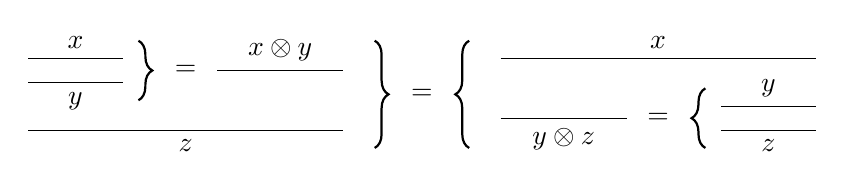
\begin{tikzpicture}[y=1ex,decoration={brace, amplitude=5pt}]
	\draw (0,0) to node[above] (x) {$x$} +(1.2,0);
	\draw (0,-2) to node[below] (y) {$y$} +(1.2,0);
	\draw[decorate, thick] (1.4,1.5) -- (1.4,-3.5);
	\node at (2, -1) (eq1) {=};
	\draw (2.4, -1) to node[above] (xy) {$x\otimes y$} (4,-1);
	\draw (0,-6) to node[below] (z) {$z$} (4,-6);
	\draw[decorate, thick] (4.4, 1.5) -- (4.4, -7.5);
	\node at (5, -3) (eq2) {=};
	\draw[decorate, thick] (5.6, -7.5) -- (5.6, 1.5);
	\draw (6, 0) to node[above] (x1) {$x$} (10,0);
	\draw (6, -5) to node[below] (yz) {$y\otimes z$} (7.6, -5);
	\node at (8, -5) (eq3) {=};
	\draw[decorate, thick] (8.6, -7.5) -- (8.6, -2.5);
	\draw (8.8, -4) to node[above] {$y$} + (1.2,0);
	\draw (8.8, -6) to node[below] {$z$} + (1.2,0);
\end{tikzpicture}
\]
But this looks much harder than it is: the associative property should be
thought of as saying that there is no distinction between the stuff on the very
left above and the stuff on the very right, i.e.\ %
\index{associativity!in wiring diagrams}
\[
\begin{tikzpicture}[y=1ex,decoration={brace, amplitude=5pt}]
	\draw (0,0) to node[above] (x) {$x$} +(1.2,0);
	\draw (0,-2) to node[below] (y) {$y$} +(1.2,0);
	\draw (0,-6) to node[below] (z) {$z$} +(1.2,0);
	\node at (5, -3) (eq2) {=};
	\draw (8.8, 0) to node[above] (x1) {$x$} +(1.2,0);
	\draw (8.8, -4) to node[above] {$y$} + (1.2,0);
	\draw (8.8, -6) to node[below] {$z$} + (1.2,0);
\end{tikzpicture}
\]
and indeed a diagram that moves from one to the other is valid.
%\[
%\begin{tikzpicture}[oriented WD, y=1ex,decoration={brace, amplitude=5pt}]
%	\draw (0,0) to node[above] (x) {$x$} +(1.2,0);
%	\draw (0,-2) to node[below] (y) {$y$} +(1.2,0);
%	\draw (0,-6) to node[below] (z) {$z$} +(1.2,0);
%	\draw (1.2,0) to (4,0);
%	\draw (1.2,-2) to (4,-4);
%	\draw (1.2,-6) to (4,-6);
%	\draw (4, 0) to node[above] (x1) {$x$} +(1.2,0);
%	\draw (4, -4) to node[above] {$y$} + (1.2,0);
%	\draw (4, -6) to node[below] {$z$} + (1.2,0);
%\end{tikzpicture}
%\]

Finally, the symmetry condition (d), that $x\otimes y = y\otimes x$, says that a
diagram is valid even if its wires cross:
%\[
%\begin{tikzpicture}[oriented WD, font=\small]
%	\node[bb={2}{2}] (xy) {};
%	\node[bb={2}{2}, right=2 of xy] (yx) {};
%	\node[left] at (xy_in1) {$x$};
%	\node[left] at (xy_in2) {$y$};
%	\node[left] at (yx_in1) {$y$};
%	\node[left] at (yx_in2) {$x$};
%	\node[right] at (xy_out1) {$y$};
%	\node[right] at (xy_out2) {$x$};
%	\node[right] at (yx_out1) {$x$};
%	\node[right] at (yx_out2) {$y$};
%\end{tikzpicture}
%\]
%but in practice it is easier to see what is going on if we denote these axiomatically-guaranteed boxes without a box at all, but instead by simply drawing wires crossing:
\[
\begin{tikzpicture}[oriented WD, font=\small]
	\node[bb={2}{2}, color=white] (xy) {};
	\node[bb={2}{2}, color=white, right=2 of xy] (yx) {};
	\node[left=2pt] at (xy_in1') (x11) {$x$};
	\node[left=2pt] at (xy_in2') (y11) {$y$};
	\node[right=2pt] at (xy_out1') (y12) {$y$};
	\node[right=2pt] at (xy_out2') (x12) {$x$};
	\node[left=2pt] at (yx_in1') (y21){$y$};
	\node[left=2pt] at (yx_in2') (x21){$x$};
	\node[right=2pt] at (yx_out1') (x22) {$x$};
	\node[right=2pt] at (yx_out2') (y22) {$y$};
	\draw (x11) to (x12);
	\draw (y11) to (y12);
	\draw (x21) to (x22);
	\draw (y21) to (y22);
\end{tikzpicture}
\]
One may regard the pair of crossing wires as another icon in our iconography, in addition to the boxes and wires we already have.%
\index{wiring diagram!icon of}%
\index{icon!crossing wires}%
\index{symmetry!in wiring diagrams}

\paragraph{Wiring diagrams as graphical proofs}%
\index{wiring diagram!as graphical proof}

Given a monoidal preorder $\cat{X}=(X,\leq, I, \otimes)$, a wiring diagram is a graphical proof of something about $\cat{X}$. Each box in the diagram has a left side and a right side, say $x$ and $y$, and represents the assertion that $x\leq y$.
\[
\begin{tikzpicture}[oriented WD]
	\node[bb={1}{1}] (f) {$\leq$};
	\draw (f_in1) to node[below] {$x$} +(-1,0);
	\draw (f_out1) to node[below] {$y$} +(1,0);
\end{tikzpicture}
\]
A wiring diagram is a bunch of interior boxes connected together inside an exterior box. It represents a graphical proof that says: if all of the interior assertions are correct, then so is the exterior assertion.
\begin{equation}%
\label{eqn.random5739_string_diag}
  \begin{aligned}
\begin{tikzpicture}[oriented WD, font=\small]
	\node[bb={1}{2}] (A) {$\leq$};
	\node[bb={2}{2}, below right=-1 and 1 of A] (B) {$\leq$};
	\node[bb={2}{1}, above right=-1 and 1 of B] (C) {$\leq$};
	\node[bb={0}{0}, fit=(A) (B) (C)] (Y) {};
	\draw (Y.west|-A_in1) to node[above] {$t$} (A_in1);
	\draw (Y.west|-B_in2) to node[below] {$u$} (B_in2);
	\draw (A_out1) to node[above] {$v$} (C_in1);
	\draw (A_out2) to node[above] {$w$} (B_in1);
	\draw (B_out1) to node[above] {$x$} (C_in2);	
	\draw (C_out1) to node[above] {$y$} (C_out1-|Y.east);
	\draw (B_out2) to node[below] {$z$} (B_out2-|Y.east);
\end{tikzpicture}
\end{aligned}
\end{equation}
The inner boxes in \cref{eqn.random5739_string_diag} translate into the assertions:
\begin{equation}%
\label{eqn.some_random334_assertions}
	t\leq v+w\qquad w+u\leq x+z\qquad v+x\leq y
\end{equation}
and the outer box translates into the assertion:
\begin{equation}%
\label{eqn.random334_conclusion}
	t+u\leq y+z.
\end{equation}
The whole wiring diagram \ref{eqn.random5739_string_diag} says ``if you know
that the assertions in \ref{eqn.some_random334_assertions} are true, then I am a
proof that the assertion in \ref{eqn.random334_conclusion} is also true.'' What
exactly is the proof that diagram \ref{eqn.random5739_string_diag} represents? It is
the proof
\begin{equation}%
\label{eqn.almost_proof}
	t+u\;\leq\; v+w+u\;\leq\;v+x+z\;\leq\; y+z.
\end{equation}
Indeed, each inequality here is a vertical slice of the diagram
\ref{eqn.random5739_string_diag}, and the transitivity of these inequalities is
expressed by connecting these vertical slices together.

\begin{example}%
\index{pie!lemon meringue}
Recall the lemon meringue pie wiring diagram from \cref{eqn.how_to_bake_pie}. It has five interior boxes, such as ``separate egg'' and ``fill crust,'' and it has one exterior box called ``prepare lemon meringue pie.'' Each box is the assertion that, given the collection of resources on the left, say an egg, you can transform it into the collection of resources on the right, say an egg white and an egg yolk. The whole string diagram is a proof that if each of the interior assertions is true---i.e.\ you really do know how to separate eggs, make lemon filling, make meringue, fill crust, and add meringue---then the exterior assertion is true: you can prepare a lemon meringue pie. 
\end{example}

\begin{exercise} %
\label{exc.proof_by_wiring}
The string of inequalities in \cref{eqn.almost_proof} is not quite a proof, because technically there is no such thing as $v+w+u$, for example. Instead, there is $(v+w)+u$ and $v+(w+u)$, and so on.
\begin{enumerate}
	\item Formally prove, using only the rules of symmetric monoidal preorders (\cref{def.symm_mon_structure}), that given the assertions in \cref{eqn.some_random334_assertions}, the conclusion in \cref{eqn.random334_conclusion} follows.
	\item Reflexivity and transitivity should show up in your proof. Make sure you are explicit about where they do.
	\item How can you look at the wiring diagram
	\cref{eqn.random334_string_diag} and know that the symmetry axiom
	(\cref{def.symm_mon_structure}(d)) does not need to be invoked?
\qedhere
\end{enumerate}
\end{exercise}

%
\index{wiring diagram|)}

We next discuss some examples of symmetric monoidal preorders. We begin in
\cref{subsec.SMPs_science} with some more concrete examples, from science, commerce, and informatics. Then in \cref{subsec.SMPs_pure_math} we discuss some examples arising from pure math, some of which will get a good deal of use later on, e.g.\ in \cref{chap.codesign}.

%---- Subsection ----%
\subsection{Applied examples}%
\label{subsec.SMPs_science}

Resource theories are studies of how resources are exchanged in a given arena. For example, in social resource theory one studies a marketplace where combinations of goods can be traded for---as well as converted into---other combinations of goods.

Whereas marketplaces are very dynamic, and an apple might be tradable for an orange on Sunday but not on Monday, what we mean by resource theory in this chapter is a static notion: deciding ``what buys what,'' once and for all.% 
\footnote{Using some sort of temporal theory, e.g.\ the one presented in \cref{chap.temporal_topos}, one could take the notion here and have it change in time.}
This sort of static notion of conversion might occur in chemistry: the chemical reactions that are possible one day will quite likely be possible on a different day as well. Manufacturing may be somewhere in between: the set of production techniques---whereby a company can convert one set of resources into another---do not change much from day to day.

We learned about resource theories from
\cite{Coecke.Fritz.Spekkens:2016a,Fritz:2017a}, who go much further than we
will; see \cref{sec.resource_theory_further_reading} for more information.%
\index{resource!theory} In
this section we will focus only on the main idea. While there are many beautiful
mathematical examples of symmetric monoidal preorders, as we will see in
\cref{subsec.SMPs_pure_math}, there are also ad hoc examples coming from life
experience. In the next chapter, on databases, we will see the same theme: while
there are some beautiful mathematical categories out there, database schemas are
\emph{ad hoc} organizational patterns of information. Describing something as
``ad hoc'' is often considered derogatory, but it just means ``formed, arranged,
or done for a particular purpose only.'' There is nothing wrong with doing
things for a particular purpose; it's common outside of pure math and pure art. Let's get
to it.

% Subsubsection %
\paragraph{Chemistry}%
\label{subsubsec.chemistry}%
\index{chemistry!monoidal preorder of}

In high school chemistry, we work with chemical equations, where material collections such as
\[\mathrm{H_2O},\quad \mathrm{NaCl},\quad \mathrm{2NaOH},\quad \mathrm{CH_4+3O_2}\]
are put together in the form of reaction equations, such as
\[\mathrm{2H_2O+2Na\to 2NaOH+H_2}.\]
The collection on the left, $\mathrm{2H_2O+2Na}$ is called the \emph{reactant}, and the collection on the right, $\mathrm{2NaOH+H_2}$ is called the \emph{product}.

We can consider reaction equations such as the one above as taking place inside a single symmetric monoidal preorder $(\Set{Mat},\to,0,+)$. Here $\Set{Mat}$ is the set of all collections of atoms and molecules, sometimes called \emph{materials}. So we have $\mathrm{NaCl}\in\Set{Mat}$ and $\mathrm{4H_2O+6Ne}\in\Set{Mat}$.

The set $\Set{Mat}$ has a preorder structure denoted by the $\to$ symbol, which is the preferred symbol in the setting of chemistry. To be clear, $\to$ is taking the place of the order relation $\leq$ from \cref{def.symm_mon_structure}. The $+$ symbol is the preferred notation for the monoidal product in the chemistry setting, taking the place of $\otimes$. While it does not come up in practice, we use $0$ to denote the monoidal unit.

\begin{exercise} %
\label{exc.reaction_equations}
Here is an exercise for people familiar with reaction equations: check that
conditions (a), (b), (c), and (d) of \cref{def.symm_mon_structure} hold.
\end{exercise}

%
\index{chemistry!catalysis}
An important notion in chemistry is that of catalysis: one compound \emph{catalyzes} a certain reaction. For example, one might have the following set of reactions:
\begin{equation}%
\label{eqn.three_reactions}
  y+k\to y'+k'\qquad x+y'\to z'\qquad z'+k'\to z+k
\end{equation}
Using the laws of monoidal preorders, we obtain the composed reaction
\begin{equation}%
\label{eqn.result_reaction}
	x+y+k\to x+y'+k'\to z'+k'\to z+k.
\end{equation}
Here $k$ is the catalyst because it is found both in the reactant and the product of the reaction. It is said to catalyze the reaction $x+y\to z$. The idea is that the reaction $x+y\to z$ cannot take place given the reactions in \cref{eqn.three_reactions}. But if $k$ is present, meaning if we add $k$ to both sides, the resulting reaction can take place.

The wiring diagram for the reaction in \cref{eqn.result_reaction} is shown in \cref{eqn.catalyst}. The three interior boxes correspond to the three reactions given in \cref{eqn.three_reactions}, and the exterior box corresponds to the composite reaction $x+y+k\to z+k$.
\begin{equation}%
\label{eqn.catalyst}
\begin{tikzpicture}[oriented WD, bbx=1cm, font=\tiny, baseline=(a)]
	\node[bb={2}{2}] (a1) {$\to$};
	\node[bb={2}{1}, above right=-1.5 and 1 of a1] (a2) {$\to$};
	\node[bb={2}{2}, below right=-1.5 and 1 of a2] (a3) {$\to$};
	\node[bb={0}{0}, fit=(a1) (a2) (a3)] (a) {};
	\draw (a.west|-a1_in1) to node[above] {$y$} (a1_in1);
	\draw (a.west|-a1_in2) to node[below] {$k$} (a1_in2);
	\draw (a.west|-a2_in1) to node[above] {$x$} (a2_in1);
	\draw (a1_out1) to node[above] {$y'$} (a2_in2);
	\draw (a1_out2) to node[below] {$k'$} (a3_in2);
	\draw (a2_out1) to node[above=3pt] {$z'$} (a3_in1);
	\draw (a3_out1) to node[above] {$z$} (a3_out1-|a.east);
	\draw (a3_out2) to node[below] {$k$} (a3_out2-|a.east);
\end{tikzpicture}
\end{equation}

\paragraph{Manufacturing}%
\label{subsubsec.manufacturing}
%
\index{manufacturing!monoidal preorder of}

Whether we are talking about baking pies, building smart phones, or following pharmaceutical recipes, manufacturing firms need to store basic recipes, and build new recipes by combining simpler recipes in schemes like the one shown in \cref{eqn.how_to_bake_pie} or \cref{eqn.catalyst}.

The basic idea in manufacturing is exactly the same as that for chemistry, except there is an important assumption we can make in manufacturing that does not hold for chemical reactions:
\begin{center}
\emph{You can trash anything you want, and it disappears from view.}
\end{center}
This simple assumption has caused the world some significant problems, but it is
still in effect. In our meringue pie example, we can ask: ``what happened to the
egg shell, or the paper wrapping the stick of butter''? The answer is they were
trashed, i.e.\ thrown in the garbage bin. It would certainly clutter our diagram
and our thinking if we had to carry these resources through the diagram:
\[
\begin{tikzpicture}[oriented WD, align=center, bbx=1.2cm, bby=2ex]
	\node[bb={4}{3}, bb min width=.9in] (filling) {make\\lemon\\filling};
	\node[bb={2}{1}, bb min width=.9in, below=of filling] (meringue) {make\\meringue};
	\node at ($(filling.south west)!.5!(meringue.north west)$) (helper) {};
	\node[bb port sep=1, bb={1}{3}, left = of helper] (separate) {separate\\egg};
	\node[bb={2}{1}, above right = -2 and 1 of filling] (fill) {fill crust};
	\node[bb={2}{1}, below right = of fill] (finish) {add\\meringue};
	\node[bb={0}{0}, bb name={prepare lemon meringue pie, keeping track of waste}, fit={(separate) (meringue) ($(fill.north)+(0,2)$) (finish)}] (pie) {};
%
\begin{scope}[font=\tiny]
	\draw (pie.west|-fill_in1) to node[above] {crust} (fill_in1);
	\draw (pie.west|-filling_in1) to node[above] {lemon} (filling_in1);
	\draw (pie.west|-filling_in2) to node[above] {butter} (filling_in2);
	\draw (pie.west|-filling_in3) to node[above] {sugar} (filling_in3);
	\draw (pie.west|-separate_in1) to node[above] {egg} (separate_in1);
	\draw (pie.west|-meringue_in2) to node[above] {sugar} (meringue_in2);
	\draw (separate_out1) to node[above] {yolk} (filling_in4);
	\node[coordinate] at ($(finish.south west)+(0,-1)$) (trash 1) {};
	\node[coordinate] at ($(finish.south west)+(0,-3)$) (trash 2) {};
	\node[coordinate] at ($(finish.south west)+(0,-5)$) (trash 3) {};
	\draw[purple] let \p1=(fill.east|-separate_out2), \n1=\bbportlen in
		(separate_out2) to node[above, pos=.8] {egg shells} (\x1+\n1,\y1) to (trash 3) -- (trash 3-|pie.east);
	\draw (separate_out3) to node[fill=white, inner sep=0.8pt] {white} (meringue_in1);
	\draw (filling_out1) to node[fill=white, inner sep=0.8pt] {lemon\\filling} (fill_in2);
	\draw[purple] let \p1=(fill.east|-filling_out2), \n1=\bbportlen in
		(filling_out2) to node[above] {lemon peel} (\x1+\n1,\y1) to (trash 1) -- (trash 1-|pie.east);
	\draw[purple] let \p1=(fill.east|-filling_out3), \n1=\bbportlen in
		(filling_out3) to node[above] {butter wrapper} (\x1+\n1,\y1) to (trash 2) -- (trash 2-|pie.east);
	\draw (fill_out1) to node[fill=white, inner sep=0.8pt] {unbaked\\lemon pie} (finish_in1);
	\draw let \p1=(fill.east|-meringue_out1), \n1=\bbportlen in
		(meringue_out1) to node[above] {meringue} (\x1+\n1,\y1) to (finish_in2);
	\draw (finish_out1) to node[above] {unbaked\\pie} (finish_out1-|pie.east);
\end{scope}
\end{tikzpicture}
\]

Instead, in our daily lives and in manufacturing, we do not have to hold on to something if we don't need it; we can just discard it. In terms of wiring diagrams, this can be shown using a new icon $\begin{tikzpicture}[spider]\node[spider={1}{0}, fill=black] {};\end{tikzpicture}$, as follows:%
\index{icon!discard}%
\index{manufacturing!discard operation in}
\begin{equation}%
\label{eqn.discard}
\begin{tikzpicture}[oriented WD]
	\node[bb={1}{2}] (A) {};
	\node[bb={2}{1}, below right=-1 and 1 of A] (B) {};
	\node[bb={0}{0}, fit=(A) (B)] (outer) {};
	\node[right=.6 of A_out1] (kill) {$\bullet$};
	\draw (outer.west|-A_in1) -- (A_in1);
	\draw (outer.west|-B_in2) -- (B_in2);
	\draw (A_out1) to node[above, font=\footnotesize] {discard} (kill.center);
	\draw (A_out2) to (B_in1);
	\draw (B_out1) -- (B_out1-|outer.east);
\end{tikzpicture}
\end{equation}

To model this concept of waste using monoidal categories, one just adds an
additional axiom to (a), (b), (c), and (d) from \cref{def.symm_mon_structure}:
\bigskip
\begin{enumerate}[label=(e)]
	\item $x\leq I$ for all $x\in X$.\hfill{(discard axiom)}%
\label{page.discard_axiom}
\end{enumerate}
\bigskip
It says that every $x$ can be converted into the monoidal unit $I$. In the notation of the chemistry section, we would write instead $x\to 0$: any $x$ yields nothing. But this is certainly not accepted in the chemistry setting. For example,
\[\mathrm{H_2O+NaCl\to^?H_2O}\]
is certainly not a legal chemical equation. It is easy to throw things away in
manufacturing, because we assume that we have access to---the ability to grab onto and directly manipulate---each item produced. In
chemistry, when you have $10^{23}$ of substance $A$ dissolved in something else,
you cannot just simply discard $A$. So axiom (e) is valid in manufacturing but
not in chemistry. 

Recall that in \cref{ssec.wirdia2} we said that there were many different styles
of wiring diagrams. Now we're saying that adding the discard axiom changes the
wiring diagram style, in that it adds this new discard icon that allows wires to terminate, as shown in
\cref{eqn.discard}. In informatics, we will change the wiring diagram style yet
again.%
\index{wiring diagram!icon of}

\paragraph{Informatics}%
\label{subsubsec.informatics}
%
\index{informatics!monoidal preorder of}
A major difference between information and a physical object is that information
can be copied. Whereas one cup of butter never becomes two, it is easy for a
single email to be sent to two different people. It is much easier to copy a
music file than it is to copy a CD. Here we do not mean ``copy the information
from one compact disc onto another''---of course that's easy---instead, we mean
that it's quite difficult to copy the physical disc, thereby forming a second
physical disc! In diagrams, the distinction is between the relation
\[
\begin{tikzpicture}[oriented WD, font=\footnotesize, bb port length=0pt]
	\node[bb={2}{2}] (copycd) {copy cd};
	\coordinate [left=1 of copycd] (l);
	\coordinate [right=1 of copycd] (r);
	\node[bb={2}{2}, fit=(copycd) (l) (r)] (outer) {};
	\draw (outer_in1) to node[above] {Beyonc\'e cd} (copycd_in1|-outer_in1);
	\draw (outer_in2) to node[below] {blank cd} (copycd_in2|-outer_in2);
	\draw (copycd_out1|-outer_out1) to node[above] {Beyonc\'e cd} (outer_out1);
	\draw (copycd_out2|-outer_out2) to node[below] {Beyonc\'e cd} (outer_out2);
\end{tikzpicture}
\]%
\index{Beyonc\'e}
and the relation
\[
\begin{tikzpicture}[oriented WD, font=\footnotesize, bb port length=0pt]
	\node[bb={1}{2}, align=center] (copycd) {no, I mean\\literally copy cd!};
	\coordinate [left=1 of copycd] (l);
	\coordinate [right=1 of copycd] (r);
	\node[bb={1}{2}, fit=(copycd) (l) (r)] (outer) {};
	\draw (outer_in1) to node[above] {Beyonc\'e cd} (copycd_in1|-outer_in1);
	\draw (copycd_out1|-outer_out1) to node[above] {Beyonc\'e cd} (outer_out1);
	\draw (copycd_out2|-outer_out2) to node[below] {Beyonc\'e cd} (outer_out2);
\end{tikzpicture}
\]
The former is possible, the latter is magic.


Of course material objects can sometimes be copied; cell mitosis is a case in point. But 
this is a remarkable biological process, certainly not something that is expected for
ordinary material objects. In the physical world, we would make mitosis a box transforming one cell into two. But in (classical, not quantum) information, everything can be copied, so we add a new icon to our repertoire.%
\index{icon!copy}

Namely, in wiring diagram notation, copying information appears as a new icon, $\begin{tikzpicture}[spider, baby]\node[spider={1}{2}, fill=black] {};\end{tikzpicture}$, allowing us to split wires:%
\index{notation|seealso {icon}}
\[
\begin{tikzpicture}[oriented WD, font=\footnotesize, bb port length=0pt]
	\node[bb={2}{1}] (draft) {write};
	\node[right=.6 of draft_out1] (dup) {$\bullet$};
	\node[bb={0}{2}, fit=(draft) (dup)] (outer) {};
	\draw (outer.west|-draft_in1) to node[above] {calendar} (draft_in1);
	\draw (outer.west|-draft_in2) to node[below] {maps} (draft_in2);
	\draw (draft_out1) to node[above] {email} (dup.center);
	\draw (dup.center) to node[above=3pt] {email} (outer_out1);
	\draw (dup.center) to node[below=2pt] {email}(outer_out2);
\end{tikzpicture}
\]
Now with two copies of the email, we can send one to Alice and one to Bob.
\begin{equation}%
\label{eqn.copy_pic}
\begin{tikzpicture}[oriented WD, font=\footnotesize, bb port length=0pt]
	\node[bb={2}{1}] (draft) {write};
	\node[right=.6 of draft_out1] (dup) {$\bullet$};
	\node[bb={1}{1}, above right=.2 and .7 of dup] (alice) {send to Alice};
	\node[bb={1}{1}, below right=.2 and .7 of dup] (bob) {send to Bob};
	\coordinate [right = 1 of bob] (x);
	\node[bb={0}{2}, fit=(draft) (dup) (alice) (bob) (x)] (outer) {};
	\draw (outer.west|-draft_in1) to node[above] {calendar} (draft_in1);
	\draw (outer.west|-draft_in2) to node[below] {maps} (draft_in2);
	\draw (draft_out1) to node[above] {email} (dup.center);
	\draw (dup.center) to node[above=5pt] {email} (alice_in1);
	\draw (dup.center) to node[below=5pt] {email}(bob_in1);
	\draw (alice_out1) to node[above] {email sent to Alice}
	(outer_out1|-alice_out1);
	\draw (bob_out1) to node[below] {email sent to Bob} (outer_out2|-bob_out1);
\end{tikzpicture}
\end{equation}

Information can also be discarded, at least in the conventional way of thinking,
so in addition to axioms (a) to (d) from \cref{def.symm_mon_structure}, we can
keep axiom (e) from page~\pageref{page.discard_axiom} and add a new \emph{copy axiom}:
\bigskip
\begin{enumerate}[label=(f)]
	\item $x\leq x+x$ for all $x\in X$.\hfill{(copy axiom)}%
\label{page.copy_axiom}
\end{enumerate}
\bigskip
allowing us to make mathematical sense of diagrams like \cref{eqn.copy_pic}.%
\index{informatics!duplication in}%
\index{informatics!discarding in}

Now that we have examples of monoidal preorders under our belts, let's discuss some
nice mathematical examples.

%
\index{resource!theory|)}
%---- Subsection ----%
\subsection{Abstract examples}%
\label{subsec.SMPs_pure_math}

In this section we discuss several mathematical examples of symmetric monoidal structures on preorders.

\paragraph{The Booleans}

The simplest nontrivial preorder is the booleans: $\BB=\{\true,\false\}$ with $\false\leq\true$. There are two different symmetric monoidal structures on it.

\begin{example}[Booleans with AND]%
\label{ex.Bool}%
\index{booleans!usual monoidal structure}
We can define a monoidal structure on $\BB$ by letting the monoidal unit be $\true$ and the monoidal product be $\wedge$ (AND). If one thinks of $\false=0$ and $\true=1$, then $\wedge$ corresponds to the usual multiplication operation $*$. That is, with this correspondence, the two tables below match up:
\begin{equation}%
\label{eqn.wedge_mult_table}
\begin{array}{c | c c}
	\wedge&\false&\true\\\hline
	\false&\false&\false\\
	\true&\false&\true
\end{array}
\hspace{1in}
\begin{array}{c | c c}
	*&0&1\\\hline
	0&0&0\\
	1&0&1
\end{array}
\end{equation}

One can check that all the properties in \cref{def.symm_mon_structure} hold, so we have a monoidal preorder which we denote $\Bool\coloneqq(\BB,\leq,\true,\wedge)$.
\end{example}

$\Bool$ will be important when we get to the notion of enrichment. Enriching in a monoidal preorder $\cat{V}=(V,\leq,I,\otimes)$ means ``letting $\cat{V}$ structure the question of getting from $a$ to $b$.'' All of the structures of a monoidal preorder---i.e.\ the set $V$, the ordering relation $\leq$, the monoidal unit $I$, and the monoidal product $\otimes$---play a role in how enrichment works.

For example, let's look at the case of $\Bool=(\BB,\leq,\true,\wedge)$. The fact that its underlying set is $\BB=\{\false,\true\}$ will translate into saying that ``getting from $a$ to $b$ is a $\true/\false$ question.'' The fact that $\true$ is the monoidal unit will translate into saying ``you can always get from $a$ to $a$.'' The fact that $\wedge$ is the monoidal product will translate into saying ``if you can get from $a$ to $b$ AND you can get from $b$ to $c$ then you can get from $a$ to $c$.'' Finally, the ``if-then'' form of the previous sentence is coming from the order relation $\leq$. We will make this more precise in \cref{sec.enrichment}.

We will be able to play the same game with other monoidal preorders, as we will see after we define a monoidal preorder called $\Cost$ in \cref{ex.Lawveres_base}.

\paragraph{Some other monoidal preorders}

It is a bit imprecise to call $\Bool$ ``the'' boolean monoidal preorder, because
there is another monoidal structure on $(\BB,\leq)$, which we describe in
\cref{exc.boolean_mon_pos_II}. The first structure, however, seems to be more useful in practice than the second.

\begin{exercise}%
\label{exc.boolean_mon_pos_II}%
\index{booleans!alternative
  monoidal structure}
Let $(\BB,\leq)$ be as above, but now consider the monoidal product to be $\vee$ (OR). 
\[
\begin{array}{c | c c}
	\vee&\false&\true\\\hline
	\false&\false&\true\\
	\true&\true&\true
\end{array}
\hspace{1in}
\begin{array}{c | c c}
	\max&0&1\\\hline
	0&0&1\\
	1&1&1
\end{array}
\]
What must the monoidal unit be in order to satisfy the conditions of \cref{def.symm_mon_structure}? 

Does it satisfy the rest of the conditions?
\end{exercise}

In \cref{ex.nats_with_plus,exc.monoidal_naturals} we give two different monoidal structures on the preorder $(\NN,\leq)$ of natural numbers, where $\leq$ is the usual ordering ($0\leq 1$ and $5\leq 16$). 

\begin{example}[Natural numbers with
  addition]%
\label{ex.nats_with_plus}%
\index{natural numbers}
There is a monoidal structure on $(\NN,\leq)$ where the monoidal unit is $0$ and the monoidal product is $+$, i.e.\ $6+4=10$. It is easy to check that $x_1\leq y_1$ and $x_2\leq y_2$ implies $x_1+x_2\leq y_1+y_2$, as well as all the other conditions of \cref{def.symm_mon_structure}.
\end{example}

\begin{exercise} %
\label{exc.monoidal_naturals}
Show there is a monoidal structure on $(\NN,\leq)$ where the monoidal product is $*$, i.e.\ $6*4=24$. What should the monoidal unit be?
\end{exercise}

\begin{example}[Divisibility and multiplication]
Recall from \cref{ex.orders_on_N} that there is a ``divisibility'' order on $\NN$: we write $m|n$ to mean that $m$ divides into $n$ without remainder. So $1\vert m$ for all $m$ and $4\vert 12$.

There is a monoidal structure on $(\NN,\vert\;)$, where the monoidal unit is $1$ and the monoidal product is $*$, i.e.\ $6*4=24$. Then if $x_1\vert y_1$ and $x_2\vert y_2$, then $(x_1*x_2)\vert (y_1*y_2)$. Indeed, if there is some $p_1,p_2\in\NN$ such that $x_1*p_1=y_1$ and $x_2*p_2=y_2$, then $(p_1*p_2)*(x_1*x_2)=y_1*y_2$.
\end{example}

\begin{exercise} %
\label{exc.monoidal_naturals2}
Again taking the divisibility order $(\NN,\vert\;)$. Someone proposes $0$ as the monoidal unit and $+$ as the monoidal product. Does that proposal satisfy the conditions of \cref{def.symm_mon_structure}? Why or why not?
\end{exercise}

\begin{exercise}%
\label{exc.no_maybe_yes}%
\index{Hasse diagram}
Consider the preorder $(P,\leq)$ with Hasse diagram \fbox{$\const{no}\to\const{maybe}\to\const{yes}$}. We propose a monoidal structure with $\const{yes}$ as the monoidal unit and ``min'' as the monoidal product.
\begin{enumerate}
	\item Make sense of ``$\min$'' by filling in the multiplication table with elements of $P$.
\[
\begin{array}{c|ccc}
	\min&\const{no}&\const{maybe}&\const{yes}\\\hline
	\const{no}&\?&\?&\?\\
	\const{maybe}&\?&\?&\?\\
	\const{yes}&\?&\?&\?
\end{array}
\]
	\item Check the axioms of \cref{def.symm_mon_structure} hold for $\Cat{NMY}\coloneqq(P,\leq,\const{yes},\min)$, given your definition of $\min$. If not, change your definition of $\min$.
\qedhere
\end{enumerate}
\end{exercise}



\begin{exercise}%
\label{exc.powerset_symm_mon_pos}%
\index{power set}%
\index{power set|seealso {preorder, of subobjects}}
\index{relation!subset}
Let $S$ be a set and let $\powset(S)$ be its power set, the set of all subsets of
$S$, including the empty subset, $\varnothing\ss S$, and the ``everything''
subset, $S\ss S$. We can give $\powset(S)$ an order: $A\leq B$ is given by the
subset relation $A\ss B$, as discussed in \cref{ex.powerset}. We propose a
symmetric monoidal structure on $\powset(S)$ with monoidal unit $S$ and monoidal product given by intersection $A\cap B$.%
\index{intersection}

Does it satisfy the conditions of \cref{def.symm_mon_structure}?
\end{exercise}

\begin{exercise}%
\label{exc.propositions_preorder}%
\index{proposition}%
\index{proposition|seealso {logic}}
Let $\Prop^{\NN}$ denote the set of all mathematical statements one can make
about a natural number, where we consider two statements to be the same if one
is true if and only if the other is true. For example ``$n$ is prime'' is an
element of $\Prop^\NN$, and so are ``$n=2$'' and ``$n\geq 11$.'' The statements
``$n+2=5$'' and ``$n$ is the least odd prime'' are considered the same. Given
$P,Q\in\Prop^\NN$, we say $P\leq Q$ if for all $n\in\NN$, whenever $P(n)$ is
true, so is $Q(n)$.

Define a monoidal unit and a monoidal product on $\Prop^\NN$ that satisfy the
conditions of \cref{def.symm_mon_structure}.
\end{exercise}

\paragraph{The monoidal preorder $\Cost$}

As we said above, when we enrich in monoidal preorders we see them as different ways to structure the question of ``getting from here to there.'' We will explain this in more detail in \cref{sec.enrichment}. The following monoidal preorder will eventually structure a notion of distance or cost for getting from here to there.

\begin{example}[Lawvere's monoidal
  preorder, $\Cost$]%
\label{ex.Lawveres_base}%
\index{Cost@$\Cost$}
Let $[0,\infty]$ denote the set of nonnegative real numbers---such as $0$, $1$, $15.33\ol{3}$, and $2\pi$---together with $\infty$. Consider the preorder $([0,\infty],\geq)$, with the usual notion of $\geq$, where of course $\infty\geq x$ for all $x\in[0,\infty]$.

There is a monoidal structure on this preorder, where the monoidal unit is $0$ and the monoidal product is $+$. In particular, $x+\infty=\infty$ for any $x\in[0,\infty]$. Let's call this monoidal preorder
\[
\Cost\coloneqq([0,\infty],\geq,0,+),
\]
because we can think of the elements of $[0,\infty]$ as costs. In terms of structuring
``getting from here to there,'' $\Cost$ seems to say ``getting
from $a$ to $b$ is a question of cost.'' The monoidal unit being $0$ will
translate into saying that you can always get from $a$ to $a$ at no cost. The
monoidal product being $+$ will translate into saying that the cost of getting
from $a$ to $c$ is at most the cost of getting from $a$ to $b$ \emph{plus} the cost of getting from $b$ to $c$. Finally, the ``at most'' in the previous sentence is coming from the $\geq$.
\end{example}

\paragraph{The opposite of a monoidal preorder}

One can take the opposite of any preorder, just flip the order: $(X,\leq)\op\coloneqq(X,\geq)$; see \cref{ex.opposite}. \cref{prop.opposite_monoidal_preorder} says that if the preorder had a symmetric monoidal structure, so does its opposite.

\begin{proposition}%
\label{prop.opposite_monoidal_preorder}%
\index{monoidal preorder!opposite of}
  Suppose $\cat{X}=(X,\leq)$ is a preorder and $\cat{X}\op=(X,\geq)$ is its opposite. If $(X,\leq,I,\otimes)$ is a symmetric monoidal preorder then so is its opposite, $(X,\geq,I,\otimes)$.
\end{proposition}
\begin{proof}
  Let's first check monotonicity. Suppose $x_1\geq y_1$ and $x_2\geq y_2$ in
  $\cat{X}\op$; we need to show that $x_1\otimes x_2\geq y_1\otimes y_2$. But by
  definition of opposite order, we have $y_1\leq x_1$ and $y_2\leq x_2$ in
  $\cat{X}$, and thus $y_1\otimes y_2\leq x_1\otimes x_2$ in $\cat{X}$. Thus
  indeed $x_1\otimes x_2\geq y_1\otimes y_2$ in $\cat{X}\op$. The other three
  conditions are even easier; see \cref{exc.complete_op_proof}.
\end{proof}

\begin{exercise}%
\label{exc.complete_op_proof}
  Complete the proof of \cref{prop.opposite_monoidal_preorder} by proving that the three remaining conditions of \cref{def.symm_mon_structure} are satisfied.
\end{exercise}

\begin{exercise} %
\label{exc.costop}
  Since $\Cost$ is a symmetric monoidal preorder, \cref{prop.opposite_monoidal_preorder} says that $\Cost\op$ is too.
  \begin{enumerate}
    \item What is $\Cost\op$ as a preorder?
    \item What is its monoidal unit?
    \item What is its monoidal product?
  \qedhere
\end{enumerate}
\end{exercise}

%==== Subsection ====%
\subsection{Monoidal monotone maps}%
\index{monoidal monotone|(}
Recall from \cref{ex:part_from_preorder} that for any preorder $(X,\leq)$, there is
an induced equivalence relation $\cong$ on $X$, where $x\cong x'$ iff both
$x\leq x'$ and $x'\leq x$.%
\index{equivalence relation!generated by a preorder}

\begin{definition}%
\label{def.monoidal_functor}
Let $\cat{P}=(P,\leq_P, I_P, \otimes_P)$ and $\cat{Q}=(Q,\leq_Q, I_Q,\otimes_Q)$
be monoidal preorders. A \emph{monoidal monotone} from $\cat{P}$ to $\cat{Q}$ is a
monotone map $f\colon(P,\leq_P)\to (Q,\leq_Q)$, satisfying two conditions:
\begin{enumerate}[label=(\alph*)]
	\item $I_Q\leq_Q f(I_P)$, and
	\item $f(p_1)\otimes_Qf(p_2)\leq_Q f(p_1\otimes_Pp_2)$
\end{enumerate}
for all $p_1,p_2\in P$.

There are strengthenings of these conditions that are also important. If $f$
satisfies the following conditions, it is called a \emph{strong monoidal
monotone}:
\begin{enumerate}[label=(\alph*')]
	\item $I_Q\cong f(I_P)$, and
	\item $f(p_1)\otimes_Qf(p_2)\cong f(p_1\otimes_Pp_2)$;
\end{enumerate}
and if it satisfies the following conditions it is called a \emph{strict
monoidal monotone}:
\begin{enumerate}[label=(\alph*'')]
	\item $I_Q= f(I_P)$, and
	\item $f(p_1)\otimes_Qf(p_2)= f(p_1\otimes_Pp_2)$.
\end{enumerate}
\end{definition}

Monoidal monotones are examples of \emph{monoidal functors}%
\index{monoidal functor!monoidal monotone as}, which we will see various incarnations of throughout the book; see \cref{roughdef.monoidal_functor}. What we call monoidal monotones could also be called \emph{lax monoidal monotones}, and there is a dual notion of \emph{oplax monoidal monotones}, where the inequalities in (a) and (b) are reversed; we will not use oplaxity in this book.%
\index{dual!of lax monoidal monotone}

%\begin{definition}%
\label{def.equiv_iso_mon_preorders}
%A monoidal monotone $f\colon\cat{P}\to\cat{Q}$ is called an \emph{equivalence}, if there exists $g\colon\cat{Q}\to\cat{P}$ such that $g(f(p))\cong p$ and $f(g(q))\cong q$ for every $p\in P$ and $q\in Q$.
%
%The monotone $f$ is called an \emph{isomorphism} if the two $\cong$'s above are replaced by $=$'s.
%\end{definition}

\begin{example}
There is a monoidal monotone $i\colon(\NN,\leq,0,+)\to(\RR,\leq,0,+)$, where $i(n)=n$ for all $n\in\NN$. It is clearly monotonic, $m\leq n$ implies $i(m)\leq i(n)$. It is even strict monoidal because $i(0)=0$ and $i(m+n)=i(m)+i(n)$.

There is also a monoidal monotone $f\colon(\RR,\leq,0,+)\to(\NN,\leq,0,+)$ going
the other way. Here $f(x)\coloneqq\floor{x}$ is the floor function, e.g.
$f(3.14)=3$. It is monotonic because $x\leq y$ implies $f(x)\leq f(y)$. Also
$f(0)=0$ and $f(x)+f(y)\leq f(x+y)$, so it is a monoidal monotone. But it is not
strict or even strong because $f(0.5)+f(0.5)\neq f(0.5+0.5)$.
\end{example}

Recall $\Bool=(\BB,\leq,\true,\wedge)$ from \cref{ex.Bool} and
$\Cost=([0,\infty],\ge,0,+)$ from \cref{ex.Lawveres_base}. There is a monoidal
monotone $g\colon\Bool\to\Cost$, given by $g(\false)\coloneqq \infty$ and
$g(\true)\coloneqq 0$.
\begin{exercise}%
\label{exc.bool_to_cost}~
\begin{enumerate}
	\item Check that the map $g\colon(\BB,\leq,\true,\wedge)\to([0,\infty],\geq,0,+)$ presented above indeed
  \begin{itemize}
  	\item is monotonic,
  	\item satisfies condition (a) of \cref{def.monoidal_functor}, and
  	\item satisfies condition (b) of \cref{def.monoidal_functor}.
  \end{itemize}
  \item Is $g$ strict?
  \qedhere
\qedhere
\end{enumerate}
\end{exercise}


\begin{exercise}%
\label{exc.bool_to_cost_inverses}
Let $\Bool$ and $\Cost$ be as above, and consider the following quasi-inverse functions $d,u\colon[0,\infty]\to\BB$ defined as follows:
\[
  d(x)\coloneqq
  \begin{cases}
  	\false&\tn{ if }x>0\\
		\true&\tn{ if } x=0
	\end{cases}
\hspace{1in}
  u(x)\coloneqq
  \begin{cases}
  	\false&\tn{ if }x=\infty\\
		\true&\tn{ if } x<\infty
	\end{cases}
\]
\begin{enumerate}
	\item Is $d$ monotonic?
	\item Does $d$ satisfy conditions (a) and (b) of \cref{def.monoidal_functor}?
	\item Is $d$ strict?
	\item Is $u$ monotonic?
	\item Does $u$ satisfy conditions (a) and (b) of \cref{def.monoidal_functor}?
	\item Is $u$ strict?
	\qedhere
\qedhere
\end{enumerate}
\end{exercise}


\begin{exercise}%
\label{exc.natural_monotone}
\begin{enumerate}
	\item Is $(\NN,\leq,1,*)$ a monoidal preorder, where $*$ is the usual multiplication of natural numbers?
	\item If not, why not? If so, does there exist a monoidal monotone $(\NN,\leq,0,+)\to(\NN,\leq,1,*)$? If not; why not? If so, find it.
	\item Is $(\zz,\leq,*,1)$ a monoidal preorder?
\qedhere
\end{enumerate}
\end{exercise}

%
\index{monoidal preorder|)}%
\index{monoidal monotone|)}

%-------- Section --------%
\section{Enrichment}%
\label{sec.enrichment}%
\index{enrichment|(}

In this section we will introduce $\cat{V}$-categories, where $\cat{V}$ is a
symmetric monoidal preorder. We will see that $\Bool$-categories are preorders, and
that $\Cost$-categories are a nice generalization of the notion of metric space.

%---- Subsection ----%
\subsection{$\cat{V}$-categories}%
\label{subsec.V_cats}%
\index{V-category@$\cat{V}$-category|see {enrichment}}

While $\cat{V}$-categories can be defined even when $\cat{V}$ is not symmetric,
i.e.\ just obeys conditions (a)--(c) of \cref{def.symm_mon_structure}, certain things don't work quite right. For example, we will see later in \cref{exc.check_enriched_prod} that the symmetry condition is necessary in order for products of $\cat{V}$-categories to exist. Anyway, here's the definition.

\begin{definition}%
\label{def.cat_enriched_mpos}%
\index{enrichment}
Let $\cat{V}=(V,\leq,I,\otimes)$ be a symmetric monoidal preorder. A \emph{$\cat{V}$-category} $\cat{X}$ consists of two constituents, satisfying two properties. To specify $\cat{X}$, 
\begin{enumerate}[label=(\roman*)]
	\item one specifies a set $\Ob(\cat{X})$, elements of which are called \emph{objects};
	\item for every two objects $x,y$, one specifies an element $\cat{X}(x,y)\in V$, called the \emph{hom-object}.%
	\tablefootnote{The word ``hom'' is short for \emph{homomorphism} and reflects the origins of this subject. A more descriptive name for $\cat{X}(x,y)$ might be \emph{mapping object}, but we use ``hom'' mainly because it is an important jargon word to know in the field.}
\end{enumerate}
%
\index{hom object}
%
\index{mapping object!see {hom object}}
%
\index{closed category!hom object in|see {hom object}}
The above constituents are required to satisfy two properties:
\begin{enumerate}[label=(\alph*)]
	\item for every object $x\in\Ob(\cat{X})$ we have $I\leq\cat{X}(x,x)$, and
	\item for every three objects $x,y,z\in\Ob(\cat{X})$, we have $\cat{X}(x,y)\otimes\cat{X}(y,z)\leq\cat{X}(x,z)$.
\end{enumerate}
We call $\cat{V}$ the \emph{base of the enrichment} for $\cat{X}$ or say that
$\cat{X}$ is \emph{enriched} in $\cat{V}$.%
\index{enrichment!base of}
\end{definition}

\begin{example} %
\label{ex.preorder_as_boolcat}%
\index{preorder!as $\Bool$-category}%
\index{enriched category!preorders as}
As we shall see in the next subsection, from every preorder we can construct
a $\Bool$-category, and vice versa. So, to get a feel for
$\cat{V}$-categories, let us consider the preorder generated by the Hasse diagram:
\begin{equation}%
\label{eqn.random_hasse91}
\begin{tikzpicture}[x=.7in, y=.3in, inner sep=5pt, baseline=(A.center)]
  	\node (a) at (0,4.5) {$t$};
  	\node (b) at (0,3) {$s$};
  	\node (c) at (-1,2) {$q$};
  	\node (d) at (1,2) {$r$};
  	\node (e) at (0,1) {$p$};
  	\node[draw, fit=(a) (b) (c) (d) (e)] (A) {};
  	\draw[->] (b) to (a);
  	\draw[->] (c) to (b);
  	\draw[->] (d) to (b);
  	\draw[->] (e) to (c);
  	\draw[->] (e) to (d);
\end{tikzpicture}
\end{equation}

How does this correspond to a $\Bool$-category $\cat{X}$? Well, the objects of
$\cat{X}$ are simply the elements of the preorder, i.e.\ $\Ob(\cat{X})=\{p,q,r,s,t\}$. Next, for
every pair of objects $(x,y)$ we need an element of $\BB=\{\false,\true\}$:
simply take $\true$ if $x \le y$, and $\false$ if otherwise. So for example,
since $s\leq t$ and $t\not\leq s$, we have $\cat{X}(s,t)=\true$ and
$\cat{X}(t,s)=\false$. Recalling from \cref{ex.Bool} that the
monoidal unit $I$ of $\Bool$ is $\true$, it's straightforward to check that
this obeys both (a) and (b), so we have a $\Bool$-category.

In general, it's sometimes convenient to represent a $\cat{V}$-category $\cat{X}$ with a
square matrix. The rows and columns of the matrix correspond to the objects of
$\cat{X}$, and the $(x,y)$th entry is simply the hom-object $\cat{X}(x,y)$. So,
for example, the above preorder in \cref{eqn.random_hasse91} can be
represented by the matrix%
\index{hom object}
\[
\begin{array}{c|ccccc}
  \rotatebox{45}{$\scriptstyle\cdot\leq\cdot$}&p&q&r&s&t\\\hline
  p&\true&\true&\true&\true&\true\\
  q&\false&\true&\false&\true&\true\\
  r&\false&\false&\true&\true&\true\\
  s&\false&\false&\false&\true&\true\\
  t&\false&\false&\false&\false&\true
\end{array}
\qedhere
\]
\end{example}

%---- Subsection ----%
\subsection{Preorders as $\Bool$-categories}%
\label{subsec.preorders_Bool_enriched}


Our colleague Peter Gates has called category theory ``a primordial ooze,'' because so much of it can be defined in terms of other parts of it. There is nowhere to rightly call the beginning, because that beginning can be defined in terms of something else. So be it; this is part of the fun.
%
\index{primordial ooze|seealso {ooze, primordial}}%
\index{ooze!primordial|see {primordial ooze}}

\begin{theorem}%
\label{thm.preorder_is_bool_cat}%
\index{preorder!as $\Bool$-category}%
\index{booleans!as base of enrichment for preorders}
There is a one-to-one correspondence between preorders and $\Bool$-categories.
\end{theorem}

Here we find ourselves in the ooze, because we are saying that preorders are the same as $\Bool$-categories, whereas $\Bool$ is itself a preorder. ``So then $\Bool$ is like... enriched in itself?'' Yes, every preorder, including $\Bool$, is enriched in $\Bool$, as we will now see.

\begin{proof}[Proof of \cref{thm.preorder_is_bool_cat}]
Let's check that we can construct a preorder from any $\Bool$-category. Since $\BB=\{\false,\true\}$, \cref{def.cat_enriched_mpos} says a
$\Bool$-category consists of two things:
\begin{enumerate}[label=(\roman*)]
	\item a set $\Ob(\cat{X})$, and
	\item for every $x,y\in \Ob(\cat{X})$ an element $\cat{X}(x,y)\in\BB$, i.e.\ either $\cat{X}(x,y)=\true$ or $\cat{X}(x,y)=\false$. 
\end{enumerate}
We will use these two things to begin forming a preorder whose elements are the objects of $\cat{X}$. So let's call the preorder $(X,\leq)$, and let $X\coloneqq\Ob(\cat{X})$. For the $\leq$ relation, let's declare $x\leq y$ iff $\cat{X}(x,y)=\true$. We have the makings of a preorder, but for it to work, the $\leq$ relation must be reflexive and transitive. Let's see if we get these from the properties guaranteed by \cref{def.cat_enriched_mpos}:
\begin{enumerate}[label=(\alph*)]
	\item for every element $x\in X$ we have $\true\leq\cat{X}(x,x)$,
	\item for every three elements $x,y,z\in X$ we have $\cat{X}(x,y)\wedge\cat{X}(y,z)\leq\cat{X}(x,z)$.
\end{enumerate}
For $b\in\Bool$, if $\true\leq b$ then $b=\true$, so the first statement says
$\cat{X}(x,x)=\true$, which means $x\leq x$. For the second statement, one can
consult \cref{eqn.wedge_mult_table}. Since $\false\leq b$ for all $b\in\BB$, the
only way statement (b) has any force is if $\cat{X}(x,y)=\true$ and $\cat{X}(y,z)=\true$, in which case it forces $\cat{X}(x,z)=\true$. This condition exactly translates as saying that $x\leq y$ and $y\leq z$ implies $x\leq z$. Thus we have obtained reflexivity and transitivity from the two axioms of $\Bool$-categories. 

In \cref{ex.preorder_as_boolcat}, we constructed a $\Bool$-category from a preorder.
We leave it to the reader to generalize this example and show that the two
constructions are inverses; see \cref{ex.preorders_as_boolcats}.
\end{proof}

\begin{exercise}%
\label{ex.preorders_as_boolcats}
  \begin{enumerate}
    \item Start with a preorder $(P,\le)$, and use it to define a $\Bool$-category as we did
      in \cref{ex.preorder_as_boolcat}. In the proof of \cref{thm.preorder_is_bool_cat} we
      showed how to turn that $\Bool$-category back into a preorder. Show that doing so,
      you get the preorder you started with. 

    \item Similarly, show that if you turn a $\Bool$-category into a preorder using the
      above proof, and then turn the preorder back into a $\Bool$-category using your
      method, you get the $\Bool$-category you started with.
      \qedhere
  \end{enumerate}
\end{exercise}

We now discuss a beautiful application of the notion of enriched categories: metric spaces.

%---- Subsection ----%
\subsection{Lawvere metric spaces} %
\label{subsec.Lawv_metric_spaces}%
\index{Lawvere metric space|(}%
\index{Lawvere metric space!as $\Cost$-category}

Metric spaces offer a precise way to describe spaces of points, each pair of
which is separated by some distance. Here is the usual definition:

\begin{definition}%
\label{def.ord_metric_space}%
\index{metric space!ordinary}
%
\index{metric space!extended}
A \emph{metric space} $(X,d)$ consists of:
\begin{enumerate}[label=(\roman*)]
	\item a set $X$, elements of which are called \emph{points}, and
	\item a function $d\colon X\times X\to\RR_{\ge 0}$, where $d(x,y)$ is called the \emph{distance between $x$ and $y$}.
\end{enumerate}	
These constituents must satisfy four properties:
\begin{enumerate}[label=(\alph*)]
	\item for every $x\in X$, we have $d(x,x)=0$,
	\item for every $x,y\in X$, if $d(x,y)=0$ then $x=y$,
	\item for every $x,y\in X$, we have $d(x,y)=d(y,x)$, and
	\item for every $x,y,z\in X$, we have $d(x,y)+d(y,z)\geq d(x,z)$.
\end{enumerate}
The fourth property is called the \emph{triangle inequality}.

If we ask instead in (ii) for a function $d\colon X \times X \to [0,\infty]= \RR_{\ge 0}
\cup \{\infty\}$, we call $(X,d)$ an \emph{extended} metric space.
\end{definition}
%
\index{triangle inequality}

The triangle inequality says that when plotting a route from $x$ to $z$, the distance is always at most what you get by choosing an intermediate point $y$ and going $x\to y\to z$.
\[
\begin{tikzpicture}[font=\small, x=.5cm, y=.5cm]
	\node (A) {$\bullet$};
	\node at ($(A.center)+(3,0)$) (B) {$\bullet$};
	\node at ($(B.center)+(3,4)$) (C) {$\bullet$};
	\node[left=0 of A] {$x$};	
	\node[right=0 of B] {$y$};	
	\node[right=0 of C] {$z$};
	\draw (A.center) to node[below] {$3$} (B.center);
	\draw (B.center) to node[below right] {$5$} (C.center);
	\draw (A.center) to node[above left] {$7.2$} (C.center);
\end{tikzpicture}
\]
It can be invoked three different ways in the above picture: $3+5\geq 7.2$, but also $5+7.2\geq 3$ and $3+7.2\geq 5$. Oh yeah, and $5+3\geq 7.2$, $7.2+5\geq 3$ and $7.2+3\geq 5$.

The triangle inequality wonderfully captures something about distance, as does
the fact that $d(x,x)=0$ for any $x$. However, the other two conditions are not
quite as general as we would like. Indeed, there are many examples of things
that ``should'' be metric spaces, but which do not satisfy conditions (b) or
(c) of \cref{def.ord_metric_space}.

For example, what if we take $X$ to be places in your neighborhood, but instead of measuring distance, you want $d(x,y)$ to measure \emph{effort} to get from $x$ to $y$. Then if there are any hills, the symmetry axiom, $d(x,y)=^? d(y,x)$, fails: it's easier to get from $x$ downhill to $y$ then to go from $y$ uphill to $x$.%
\index{effort!as metric}%
\index{symmetry!lack of for effort}

Another way to find a model that breaks the symmetry axiom is to imagine that the elements of $X$ are not points, but whole regions such as the US, Spain, and Boston. Say that the distance from region $A$ to region $B$ is understood using the setup ``I will put you in an arbitrary part of $A$ and you just have to get anywhere in $B$; what is the distance in the worst-case scenario?'' So $d(\mathrm{US}, \mathrm{Spain})$ is the distance from somewhere in the western US to the western tip of Spain: you just have to get into Spain, but you start in the worst possible part of the US for doing so.%
\index{Lawvere metric space!of regions}

\begin{exercise}%
\label{ex.regions_of_world}
Which distance is bigger under the above description, $d(\mathrm{Spain}, \mathrm{US})$ or $d(\mathrm{US}, \mathrm{Spain})$?
\end{exercise}

This notion of distance, which is strongly related to something called \emph{Hausdorff distance},%
\footnote{
The Hausdorff distance gives a metric on the set of all subsets $U\ss X$ of a given metric space $(X,d)$. One first defines
\[d_L(U,V)\coloneqq \sup_{u\in U}\underset{v \in V}{\inf\vphantom{p}}d(u,v),\]
and this is exactly the formula we intend above; the result will be a Lawvere
metric space. However, if one wants the Hausdorff distance to define a
(symmetric) metric, as in \cref{def.ord_metric_space}, one must take the above
formula and symmetrize it: $d(U,V)\coloneqq\max(d_L(U,V),d_L(V,U))$. We happen
to see the unsymmetrized notion as more interesting.
}%
\index{Hausdorff distance}
will again satisfy the triangle inequality, but it violates the symmetry condition. It also violates another condition, because $d(\mathrm{Boston},\mathrm{US})=0$. No matter where you are in Boston, the distance to the nearest point of the US is 0. On the other hand, $d(\mathrm{US},\mathrm{Boston})\neq 0$.

Finally, one can imagine a use for distances that are not finite. In terms of my effort, the distance from here to Pluto is $\infty$, and it would not be any better if Pluto was still a planet. Similarly, in terms of Hausdorff distance, discussed above, the distance between two regions is often infinite, e.g.\ the distance between $\{r\in\RR\mid r<0\}$ and $\{0\}$ as subsets of $(\RR,d)$ is infinite.

When we drop conditions (b) and (c) and allow for infinite distances, we get the following relaxed notion of metric space, first proposed by Lawvere. Recall the symmetric monoidal preorder $\Cost=([0,\infty],\geq,0,+)$ from \cref{ex.Lawveres_base}.

\begin{definition} %
\label{def.Lawvere_metric_space}%
\index{metric space!as $\Cost$-category}%
\index{enriched category!metric space as}
A \emph{Lawvere metric space} is a $\Cost$-category.
\end{definition}

This is a very compact definition, but it packs a punch. Let's work out what it means, by relating it to the usual definition of metric space. By \cref{def.cat_enriched_mpos}, a $\Cost$-category $\cat{X}$  consists of:
\begin{enumerate}[label=(\roman*)]
	\item a set $\Ob(\cat{X})$,
	\item for every $x,y\in \Ob(\cat{X})$ an element $\cat{X}(x,y)\in[0,\infty]$. 
\end{enumerate}
Here the set $\Ob(\cat{X})$ is playing the role of the set of points, and $\cat{X}(x,y)\in[0,\infty]$ is playing the role of distance, so let's write a little translator:
\[X\coloneqq\Ob(\cat{X})\qquad d(x,y)\coloneqq\cat{X}(x,y).\]
The properties of a category enriched in $\Cost$ are:
\begin{enumerate}[label=(\alph*)]
	\item $0\geq d(x,x)$ for all $x\in X$, and
	\item $d(x,y)+d(y,z)\geq d(x,z)$ for all $x,y,z\in X$.
\end{enumerate}
Since $d(x,x)\in[0,\infty]$, if $0\geq d(x,x)$ then $d(x,x)=0$. So the first
condition is equivalent to the first condition from \cref{def.ord_metric_space},
namely $d(x,x)=0$. The second condition is the triangle inequality.


\begin{example}%
\label{ex.reals_as_metric_space}%
\index{real numbers!as metric
  space}
The set $\RR$ of real numbers can be given a metric space structure, and hence a Lawvere metric space structure. Namely $d(x,y)\coloneqq|y-x|$, the absolute value of the difference. So $d(3,7)=4$.
\end{example}

\begin{exercise}%
\label{exc.finite_Lawvere}
Consider the symmetric monoidal preorder $(\RR_{\geq0},\geq,0,+)$, which is almost the same as $\Cost$, except it does not include $\infty$. How would you characterize the difference between a Lawvere metric space and a $(\RR_{\geq0},\geq,0,+)$-category in the sense of \cref{def.cat_enriched_mpos}?
\end{exercise}



\paragraph{Presenting metric spaces with weighted graphs}%
\index{metric space!presentation of}%
\index{presentation!of metric space}%
\index{Hasse diagram!weighted graph as}%
\index{Hasse diagram!for metric spaces}
Just as one can convert a Hasse diagram into a preorder, one can convert any
weighted graph---a graph whose edges are labeled with numbers $w\geq 0$---into a
Lawvere metric space. In fact, we shall consider these as graphs labelled with
elements of $[0,\infty]$, and more precisely call them $\Cost$-weighted
graphs.\footnote{This generalizes Hasse diagrams, which we could
call $\Bool$-weighted graphs---the edges of a Hasse diagram are thought of as
weighted with $\true$; we simply ignore any edges that are weighted with
$\false$, and neglect to even draw them!}%
\index{graph!weighted} 

One might think of a $\Cost$-weighted graph as describing a city with some
one-way roads (a two-way road is modeled as two one-way roads), each having some
effort-to-traverse, which for simplicity we just call length.  For example,
consider the following weighted graphs:
\begin{equation}%
\label{eqn.cities_distances}
\begin{tikzpicture}[font=\scriptsize, x=1cm, baseline=(Y)]
	\node (a) {$\LMO{A}$};
	\node[right=1 of a] (b) {$\LMO{B}$};
	\node[below=1 of a] (c) {$\LMO[under]{C}$};
	\node[right=1 of c] (d) {$\LMO[under]{D}$};
	\draw[->] (c) to node[above left=-1pt and -1pt] {3} (b);
	\draw[bend right,->] (a) to node[left] {3} (c);
	\draw[bend left,->] (d) to node[below] {6} (c);
	\draw[bend right,->] (b) to node[above] {2} (a);
	\draw[bend left,->] (b) to node[right] {5} (d);
	\node[draw, inner sep=15pt, fit=(a) (b) (c) (d)] (X) {};
	\node[left=0 of X, font=\normalsize] {$X\coloneqq$};
%
	\node[right=4 of b] (x) {$\LMO{x}$};
	\node[below=1 of x] (y) {$\LMO[under]{y}$};
	\node at ($(x)!.5!(y)+(1.5cm,0)$) (z) {$\LMO{z}$};
	\draw[bend left,->] (y) to node[left] {3} (x);
	\draw[bend left,->] (x) to node[right] {4} (y);	
	\draw[bend left,->] (x) to node[above] {3} (z);
	\draw[bend left,->] (z) to node[below right=-1pt and -1pt] {4} (y);
	\node[draw, inner sep=15pt, fit=(x) (y) (z.west)] (Y) {};
	\node[right=0 of Y, font=\normalsize] {$=:Y$};
\end{tikzpicture}
\end{equation}
Given a weighted graph, one forms a metric $d_X$ on its set $X$ of vertices by setting $d(p,q)$ to be the length of the shortest path from $p$ to $q$. For example, here is the the table of distances for $Y$
\begin{equation}%
\label{eqn.distances_Y}
\begin{array}{c|ccc}
d(\nearrow)&x&y&z\\\hline
x&0&4&3\\
y&3&0&6\\
z&7&4&0
\end{array}
\end{equation}

\begin{exercise}%
\label{exc.distance_matrix_X}%
\index{matrix!of distances}
Fill out the following table of distances in the weighted graph $X$ from \cref{eqn.cities_distances}
\[
\begin{array}{c|cccc}
  d(\nearrow)&A&B&C&D\\\hline
  A&0&\?&\?&\?\\
  B&2&\?&5&\?\\
  C&\?&\?&\?&\?\\
  D&\?&\?&\?&\?
\end{array}
\qedhere
\]
\end{exercise}

Above we converted a weighted graph $G$, e.g.\ as shown in \cref{eqn.cities_distances}, into a table of distances, but this takes a bit of thinking. There is a more direct construction for taking $G$ and getting a square matrix $M_G$, whose rows and columns are indexed by the vertices of $G$. To do so, set $M_G$ to be $0$ along the diagonal, to be $\infty$ wherever an edge is missing, and to be the edge weight if there is an edge.

For example, the matrix associated to $Y$ in \cref{eqn.cities_distances} would be
\begin{equation}%
\label{eqn.matrix_Y}
M_Y\coloneqq
\begin{array}{c|ccc}
  \nearrow&x&y&z\\\hline
  x & 0 & 4 & 3\\
  y & 3 & 0 & \infty\\
  z & \infty & 4 & 0
\end{array}
\end{equation}
As soon as you see how we did this, you'll understand that it takes no thinking
to turn a weighted graph $G$ into a matrix $M_G$ in this way. We will see later
in \cref{subsubsec.nav_matrix_mult} that the more difficult ``distance
matrices'' $d_Y$, such as \cref{eqn.distances_Y}, can be obtained from the easy
graph matrices $M_Y$, such as \cref{eqn.matrix_Y}, by repeating a certain sort of ``matrix multiplication.''

\begin{exercise}%
\label{exc.adjacency_matrix_X}%
\index{matrix}
Fill out the matrix $M_X$ associated to the graph $X$ in \cref{eqn.cities_distances}:
\[
M_X=
\begin{array}{c|cccc}
  \nearrow&A&B&C&D\\\hline
  A&0&\?&\?&\?\\
  B&2&0&\infty&\?\\
  C&\?&\?&\?&\?\\
  D&\?&\?&\?&\?
\end{array}
\qedhere
\]
\end{exercise}

%---- Subsection ----%
\subsection{$\cat{V}$-variations on preorders and metric spaces}%
\label{subsec.variations_quantale}

We have told the story of $\Bool$ and $\Cost$. But in \cref{subsec.SMPs_pure_math} we gave examples of many other monoidal preorders, and each one serves as the base of enrichment for a kind of enriched category. Which of them are useful? Something only becomes useful when someone finds a use for it. We will find uses for some and not others, though we encourage readers to think about what it would mean to enrich in the various monoidal categories discussed above; maybe they can find a use we have not explored.

\begin{exercise}%
\label{exc.NMY_cats}
Recall the monoidal preorder $\Cat{NMY}\coloneqq(P,\leq,\const{yes},\min)$ from
\cref{exc.no_maybe_yes}. Interpret what a $\Cat{NMY}$-category is.
\end{exercise}

In the next two exercises, we use $\cat{V}$-weighted graphs to construct
$\cat{V}$-categories. This is possible because we will use preorders that, like
$\Bool$ and $\Cost$, have joins.

\begin{exercise}%
\label{ex.modes_of_transport}%
\index{modes of transport}
Let $M$ be a set and let $\cat{M}\coloneqq(\powset(M),\ss,M,\cap)$ be the monoidal preorder whose elements are subsets of $M$.

Someone gives the following interpretation, ``for any set $M$, imagine it as the set of modes of transportation (e.g.\ car, boat, foot). Then an $\cat{M}$-category $\cat{X}$ tells you all the modes that will get you from $a$ all the way to $b$, for any two points $a,b\in\Ob(\cat{X})$.''
\begin{enumerate}
	\item Draw a graph with four vertices and four or five edges, each labeled with a subset of $M=\{\mathrm{car}, \mathrm{boat}, \mathrm{foot}\}$.	
	\item From this graph is it possible to construct an $\cat{M}$-category,
	where the hom-object from $x$ to $y$ is computed as follows: for each
	path $p$ from $x$ to $y$, take the intersection of the sets
	labelling the edges in $p$. Then, take the union of the these sets over
	all paths $p$ from $x$ to $y$. Write out the corresponding four-by-four
	matrix of hom-objects, and convince yourself that this is indeed an
	$\cat{M}$-category.%
\index{hom object}%
\index{union}
	\item Does the person's interpretation look right, or is it subtly mistaken somehow?
	\qedhere
\end{enumerate}
\end{exercise}


\begin{exercise}%
\label{exc.weight_limit}
Consider the monoidal preorder $\cat{W}\coloneqq(\NN\cup\{\infty\}, \leq, \infty,
\min)$.
\begin{enumerate}
	\item Draw a small graph labeled by elements of $\NN\cup\{\infty\}$. 
	\item Write out the matrix whose rows and columns are indexed by the
	nodes in the graph, and whose $(x,y)$th entry is given by the
	\emph{maximum} over all paths $p$ from $x$ to $y$ of the \emph{minimum}
	edge label in $p$.  
	\item Prove that this matrix is the matrix of hom-objects for a
	$\cat{W}$-category. This will give you a feel for how $\cat{W}$ works.%
\index{hom object!matrix of}
	\item Make up an interpretation, like that in
	\cref{ex.modes_of_transport}, for how to imagine enrichment in
	$\cat{W}$.
	\qedhere
\end{enumerate}
\erase{Weight-limit, e.g.\ for trucking.}
\end{exercise}

%
\index{Lawvere metric space|)}

%-------- Section --------%
\section{Constructions on $\cat{V}$-categories} %
\label{sec.vcat_constructions}

Now that we have a good intuition for what $\cat{V}$-categories are, we give
three examples of what can be done with $\cat{V}$-categories. The first
(\cref{subsec.change_base_mon_fun}) is known as change of base. This allows us
to use a monoidal monotone $f\colon \cat{V} \to \cat{W}$ to construct
$\cat{W}$-categories from $\cat{V}$-categories. The second construction
(\cref{subsec.enriched_functors}), that of $\cat{V}$-functors, allows us to
complete the analogy: a preorder is to a $\Bool$-category as a monotone map is to
what? The third construction (\cref{subsec.enriched_functors}) is known as a
$\cat{V}$-product, and gives us a way of combining two $\cat{V}$-categories.

%---- Subsection ----%
\subsection{Changing the base of enrichment}%
\label{subsec.change_base_mon_fun}%
\index{enrichment!change of base}
Any monoidal monotone $\cat{V}\to\cat{W}$ between symmetric monoidal preorders lets us convert $\cat{V}$-categories into $\cat{W}$-categories.

\begin{construction}%
\label{const.mon_fun_base_change}%
\index{change of base|see {enrichment, change of base}}%
\index{enrichment!change of base}
Let $f\colon\cat{V}\to\cat{W}$ be a monoidal monotone. Given a $\cat{V}$-category $\cat{C}$, one forms the associated $\cat{W}$-category, say $\cat{C}_f$ as follows.
\begin{enumerate}[label=(\roman*)]
	\item We take the same objects: $\Ob(\cat{C}_f)\coloneqq\Ob(\cat{C})$.
	\item For any $c,d\in\Ob(\cat{C})$, put $\cat{C}_f(c,d)\coloneqq f(\cat{C}(c,d))$.
\end{enumerate}
\end{construction}

This construction $\cat{C}_f$ does indeed obey the definition of a
$\cat{W}$-category, as can be seen by applying
\cref{def.monoidal_functor} (of monoidal monotone) and \cref{def.cat_enriched_mpos}
(of $\cat{V}$-category):
\begin{enumerate}[label=(\alph*)]
	\item for every $c\in\cat{C}$, we have
	  \begin{align*}
	    I_W &\leq f(I_V) \tag{$f$ is monoidal monotone}\\
	    &\leq f(\cat{C}(c,c)) \tag{$\cat{C}$ is $\cat{V}$-category}\\
	    &=\cat{C}_f(c,c) \tag{definition of $\cat{C}_f$}
	  \end{align*}
	\item for every $c,d,e\in\Ob(\cat{C})$ we have
	\begin{align*}
		\cat{C}_f(c,d)\otimes_W\cat{C}_f(d,e)&=f(\cat{C}(c,d))\otimes_Wf(\cat{C}(d,e))
		\tag{definition of $\cat{C}_f$}\\
		&\leq f\big(\cat{C}(c,d)\otimes_V\cat{C}(d,e)\big)
		\tag{$f$ is monoidal monotone}\\
		&\leq f(\cat{C}(c,e))
		\tag{$\cat{C}$ is $\cat{V}$-category}\\
		&=\cat{C}_f(c,e)
		\tag{definition of $\cat{C}_f$}
	\end{align*}
\end{enumerate}

\begin{example}
As an example, consider the function $f\colon[0,\infty]\to\{\true,\false\}$ given by
\begin{equation}%
\label{eqn.Lawv_to_Bool1}
	f(x)\coloneqq
	\begin{cases}
		\true&\tn{ if }x=0\\
		\false&\tn{ if }x>0
	\end{cases}
\end{equation}
It is easy to check that $f$ is monotonic and that $f$ preserves the monoidal
product and monoidal unit; that is, it's easy to show that $f$ is a monoidal
monotone. (Recall \cref{exc.bool_to_cost_inverses}.)

Thus $f$ lets us convert Lawvere metric spaces into preorders.%
\index{Lawvere metric space}
\end{example}

\begin{exercise} %
\label{exc.regions_preorder}
Recall the ``regions of the world'' Lawvere metric space from
\cref{ex.regions_of_world} and the text above it. We just learned that, using
the monoidal monotone $f$ in \cref{eqn.Lawv_to_Bool1},  we can convert it to a
preorder. Draw the Hasse diagram for the preorder corresponding to the regions:
US, Spain, and Boston. How could you interpret this preorder relation?
\end{exercise}

\begin{exercise} %
\label{exc.metric_to_poset}
\begin{enumerate}
	\item Find another monoidal monotone $g\colon\Cost\to\Bool$ different from the one defined in \cref{eqn.Lawv_to_Bool1}.
	\item Using \cref{const.mon_fun_base_change}, both your monoidal
	monotone $g$ and the monoidal monotone $f$ in \cref{eqn.Lawv_to_Bool1}
	can be used to convert a Lawvere metric space into a preorder. Find a
	Lawvere metric space $\cat{X}$ on which they give different answers,
	$\cat{X}_f\neq\cat{X}_g$.
	\qedhere
\end{enumerate}
\end{exercise}



%---- Subsection ----%
\subsection{Enriched functors} %
\label{subsec.enriched_functors}%
\index{functor!enriched|see {enriched functor}}%
\index{enriched functor}
The notion of functor provides the most important type of relationship between categories.
\begin{definition}%
\label{def.enriched_functor}
Let $\cat{X}$ and $\cat{Y}$ be $\cat{V}$-categories. A \emph{$\cat{V}$-functor from $\cat{X}$ to $\cat{Y}$}, denoted $F\colon\cat{X}\to\cat{Y}$, consists of one constituent:
\begin{enumerate}[label=(\roman*)]
	\item a function $F\colon\Ob(\cat{X})\to\Ob(\cat{Y})$
\end{enumerate}
subject to one constraint
\begin{enumerate}[label=(\alph*)]
	\item for all $x_1,x_2\in\Ob(\cat{X})$, one has $\cat{X}(x_1,x_2)\leq\cat{Y}(F(x_1),F(x_2))$.
\end{enumerate}
\end{definition}

\begin{example}%
\label{ex.bool_functors_monotone}%
\index{monotone map!as
  $\Bool$-functor}
For example, we have said several times---e.g.\ in \cref{thm.preorder_is_bool_cat}---that preorders are $\Bool$-categories, where $\cat{X}(x_1,x_2)=\true$ is denoted $x_1\leq x_2$. One would hope that monotone maps between preorders would correspond exactly to $\Bool$-functors, and that's true. A monotone map $(X,\leq_X)\to(Y,\leq_Y)$ is a function $F\colon X\to Y$ such that for every $x_1,x_2\in X$, if $x_1\leq_X x_2$ then $F(x_1)\leq_Y F(x_2)$. In other words, we have
\[\cat{X}(x_1,x_2)\leq\cat{Y}(F(x_1),F(x_2)),\]
where the above $\leq$ takes place in the enriching category $\cat{V}=\Bool$; this is exactly the condition from \cref{def.enriched_functor}.
\end{example}

\begin{remark}%
\label{rem.preorder_boolcats}%
\index{equivalence of categories}
In fact, we have what is called an \emph{equivalence} of categories between the
category of preorders and the category of $\Bool$-categories. In the next chapter
we will develop the ideas necessary to state what this means precisely
(\cref{rem.preorder_boolcats2}).
\end{remark}

\begin{example}%
\index{metric space}
Lawvere metric spaces are $\Cost$-categories. The definition of $\Cost$-functor
should hopefully return a nice notion---a ``friend''---from the theory of metric
spaces, and it does: it recovers the notion of Lipschitz function. A Lipschitz
(or more precisely, 1-Lipschitz) function is one under which the distance between any pair of points does not increase. That is, given Lawvere metric spaces $(X,d_X)$ and $(Y,d_Y)$, a $\Cost$-functor between them is a function $F\colon X\to Y$ such that for every $x_1,x_2\in X$ we have $d_X(x_1,x_2)\geq d_Y(F(x_1),F(x_2))$.
\end{example}

\begin{exercise}%
\label{def.enriched_op}%
\index{opposite!$\cat{V}$-category}
The concepts of opposite, dagger, and skeleton (see \cref{ex.opposite,ex.dagger_preorder,rem.skeletal_preorder}) extend from preorders to
$\cat{V}$-categories. The \emph{opposite} of a $\cat{V}$-category $\cat{X}$ is denoted $\cat{X}\op$
and is defined by
\begin{enumerate}[label=(\roman*)]
	\item $\Ob(\cat{X}\op)\coloneqq\Ob(\cat{X})$, and
	\item for all $x,y\in \cat{X}$, we have $\cat{X}\op(x,y)\coloneqq\cat{X}(y,x)$.
\end{enumerate}
A $\cat{V}$-category $\cat{X}$ is a \emph{dagger}%
\index{dagger}
$\cat{V}$-category if the identity function is a $\cat{V}$-functor
$\dagger\colon\cat{X}\to\cat{X}\op$.  And a  \emph{skeletal}%
\index{skeleton}
$\cat{V}$-category is one in which if $I \le \cat{X}(x,y)$ and $I \le
\cat{X}(y,x)$, then $x=y$.

Recall that an extended metric space $(X,d)$ is a Lawvere metric space with two
extra properties; see properties (b) and (c) in \cref{def.ord_metric_space}.
\begin{enumerate}
	\item Show that a skeletal dagger $\Cost$-category is an extended metric space.
	\item Use \cref{exc.skeletal_dagger_preorder} to make sense of the following analogy: ``preorders are to sets as
	Lawvere metric spaces are to extended metric spaces.''
	\qedhere
\end{enumerate}
%
%Draw the opposite of the following Lawvere-metric space.
%\[
%\begin{tikzpicture}[font=\scriptsize, x=1cm, baseline=(Y)]
%	\node (a) {$\LMO{A}$};
%	\node[right=1 of a] (b) {$\LMO{B}$};
%	\node[below=1 of a] (c) {$\LMO[under]{C}$};
%	\node[right=1 of c] (d) {$\LMO[under]{D}$};
%	\draw[->] (c) to node[above left=-1pt and -1pt] {3} (b);
%	\draw[bend right,->] (a) to node[left] {3} (c);
%	\draw[bend left,->] (d) to node[below] {6} (c);
%	\draw[bend right,->] (b) to node[above] {2} (a);
%	\draw[bend left,->] (b) to node[right] {5} (d);
%	\node[draw, inner sep=15pt, fit=(a) (b) (c) (d)] (X) {};
%	\node[left=0 of X, font=\normalsize] {$X\coloneqq$};
%\end{tikzpicture}
%\]
%Is this Lawvere metric space symmetric?
\end{exercise}

%---- Subsection ----%
\subsection{Product $\cat{V}$-categories}%
\label{subsec.enriched_products}
If $\cat{V}=(V,\leq,I,\otimes)$ is a symmetric monoidal preorder and $\cat{X}$ and $\cat{Y}$ are $\cat{V}$-categories, then we can define their $\cat{V}$-product, which is a new $\cat{V}$-category.

\begin{definition}%
\label{def.enriched_prod}%
\index{product!of $\cat{V}$-categories}
Let $\cat{X}$ and $\cat{Y}$ be $\cat{V}$-categories. Define their \emph{$\cat{V}$-product}, or simply \emph{product}, to be the $\cat{V}$-category $\cat{X}\times\cat{Y}$ with
\begin{enumerate}[label=(\roman*)]
	\item $\Ob(\cat{X}\times\cat{Y})\coloneqq\Ob(\cat{X})\times\Ob(\cat{Y})$,
	\item $(\cat{X}\times\cat{Y})\big((x,y),(x',y')\big)\coloneqq\cat{X}(x,x')\otimes\cat{Y}(y,y')$,
\end{enumerate}
for two objects $(x,y)$ and $(x',y')$ in $\Ob(\cat{X}\times\cat{Y})$. 
\end{definition}
Product $\cat{V}$-categories are indeed $\cat{V}$-categories
(\cref{def.cat_enriched_mpos}); see \cref{exc.check_enriched_prod}.

\begin{exercise}%
\label{exc.check_enriched_prod}
Let $\cat{X}\times\cat{Y}$ be the $\cat{V}$-product of $\cat{V}$-categories as in \cref{def.enriched_prod}.
\begin{enumerate}
	\item Check that for every object $(x,y)\in\Ob(\cat{X}\times\cat{Y})$ we
	have $I\leq(\cat{X}\times\cat{Y})\big((x,y),(x,y)\big)$.
	\item Check that for every three objects $(x_1,y_1)$, $(x_2,y_2),$ and $(x_3,y_3)$, we have
	\[
		(\cat{X}\times\cat{Y})\big((x_1,y_1),(x_2,y_2)\big)
		\otimes(\cat{X}\times\cat{Y})\big((x_2,y_2),(x_3,y_3)\big)
		\leq
		(\cat{X}\times\cat{Y})\big((x_1,y_1),(x_3,y_3)\big).
	\]
	\item We said at the start of \cref{subsec.V_cats} that the symmetry of $\cat{V}$ (condition (d) of \cref{def.symm_mon_structure}) would be required here. Point out exactly where that condition is used.%
\index{symmetry!as required for enriched products}
	\qedhere
\end{enumerate}
\end{exercise}


When taking the product of two preorders $(P,\leq_P)\times(Q,\leq_Q)$, as first described in \cref{ex.product_preorder}, we say that $(p_1,q_1)\leq (p_2,q_2)$ iff both $p_1\leq p_2$ AND $q_1\leq q_2$; the AND is the monoidal product $\otimes$ from of $\Bool$. Thus the product of preorders is an example of a $\Bool$-product.

\begin{example}%
\index{weighted graph|see {graph, weighted}}
Let $\cat{X}$ and $\cat{Y}$ be the Lawvere metric spaces (i.e.\ $\Cost$-categories) defined by the following weighted graphs:
\begin{equation}%
\label{eqn.weighted_graphs_XY}
\begin{tikzpicture}[font=\scriptsize, x=1cm, y=1cm, every label/.style={font=\tiny}]
	\node[label={[above=-5pt]:$A$}] (A) {$\bullet$};
	\node[right=1 of A, label={[above=-5pt]:$B$}] (B) {$\bullet$};
	\node[right=1 of B, label={[above=-5pt]:$C$}] (C) {$\bullet$};
	\draw[->] (A) to node[above] {2} (B);
	\draw[->] (B) to node[above] {3} (C);
	\node[draw, inner ysep=10pt, fit=(A) (C)] (X) {};
	\node[left=0 of X, font=\normalsize] {$\cat{X}\coloneqq$};
%
	\node[below right=.4 and 2 of C, label={[below=5pt]:$q$}] (y) {$\bullet$};
	\node[above=1 of y,label={[above=-5pt]:$p$}] (x) {$\bullet$};
%	\node[below=1 of y,label={[below=5pt]:$r$}] (z) {$\bullet$};
	\draw[->, bend right] (x) to node[left] {5} (y);
	\draw[->, bend right] (y) to node[right] {8} (x);
%	\draw[->, shorten <=6pt] (y) to node[right] {4} (z);
	\node[draw, inner sep=15pt, fit=(x) (y)] (Y) {};
%	\node[draw, inner sep=15pt, fit=(x) (z)] (Y) {};
	\node[right=0 of Y, font=\normalsize] {$=:\cat{Y}$};	
\end{tikzpicture}
\end{equation}
Their product is defined by taking the product of their sets of objects, so there are six objects in $\cat{X}\times\cat{Y}$. And the distance $d_{X\times Y}((x,y),(x',y'))$ between any two points is given by the sum $d_X(x,x')+d_Y(y,y')$.

Examine the following graph, and make sure you understand how easy it is to derive from the weighted graphs for $\cat{X}$ and $\cat{Y}$ in \cref{eqn.weighted_graphs_XY}:
\[
\begin{tikzpicture}[font=\scriptsize, x=1.4cm, y=1.4cm, every label/.style={font=\tiny}]
	\node               [label={[above=-5pt]:$(A,p)$}] (Ap) {$\bullet$};
	\node[right=1 of Ap, label={[above=-5pt]:$(B,p)$}] (Bp) {$\bullet$};
	\node[right=1 of Bp, label={[above=-5pt]:$(C,p)$}] (Cp) {$\bullet$};
	\node[below=1 of Ap, label={[below=5pt]:$(A,q)$}] (Aq) {$\bullet$};
	\node[right=1 of Aq, label={[below=5pt]:$(B,q)$}] (Bq) {$\bullet$};
	\node[right=1 of Bq, label={[below=5pt]:$(C,q)$}] (Cq) {$\bullet$};
%
	\draw[->] (Ap) to node[above] {2} (Bp);
	\draw[->] (Bp) to node[above] {3} (Cp);
	\draw[->] (Aq) to node[above] {2} (Bq);
	\draw[->] (Bq) to node[above] {3} (Cq);
%
	\draw[->, bend right] (Ap) to node[left] {5} (Aq);
	\draw[->, bend right] (Aq) to node[right] {8} (Ap);
	\draw[->, bend right] (Bp) to node[left] {5} (Bq);
	\draw[->, bend right] (Bq) to node[right] {8} (Bp);
	\draw[->, bend right] (Cp) to node[left] {5} (Cq);
	\draw[->, bend right] (Cq) to node[right] {8} (Cp);
%
	\node[draw, inner sep=15pt, fit=(Ap) (Cq)] (prod) {};
	\node[left=0 of prod, font=\normalsize] {$\cat{X}\times\cat{Y}=$};
\end{tikzpicture}
\qedhere
\]
\end{example}

\begin{exercise}%
\label{exc.not_sqrt40}
Consider $\RR$ as a Lawvere metric space, i.e.\ as a $\Cost$-category (see \cref{ex.reals_as_metric_space}). Form the $\Cost$-product $\RR\times\RR$. What is the distance from $(5,6)$ to $(-1,4)$? Hint: apply \cref{def.enriched_prod}; the answer is not $\sqrt{40}$.
\end{exercise}

In terms of matrices, $\cat{V}$-products are also quite straightforward. They generalize what is known as the Kronecker product of matrices. The matrices for $\cat{X}$ and $\cat{Y}$ in \cref{eqn.weighted_graphs_XY} are shown below
\[
\begin{array}{c|ccc}
  \cat{X}&A&B&C\\\hline
  A & 0 & 2 & 5\\
  B & \infty  & 0 & 3\\
  C & \infty & \infty & 0
\end{array}
\hspace{1in}
\begin{array}{c|cc}
  \cat{Y}&p&q\\\hline
  p & 0 & 5\\
  q & 8 & 0
\end{array}
\]
and their product is as follows:
\[
\begin{array}{c||ccc| ccc}
	\cat{X}\times\cat{Y}&(A,p)&(B,p)&(C,p)&(A,q)&(B,q)&(C,q)\\\hline\hline
	(A,p)& 0 & 2 & 5 & 5&7&10\\
	(B,p)& \infty & 0 & 3 & \infty & 5 & 8\\
	(C,p)& \infty &\infty & 0& \infty&\infty &5\\\hline
	(A,q)& 8 & 10 & 13 & 0 & 2 & 5\\
	(B,q)& \infty & 8 & 11 & \infty & 0 & 3\\
	(C,q)& \infty & \infty & 8 & \infty &\infty & 0
\end{array}
\]
We have drawn the product matrix as a block matrix, where there is one block---shaped like $\cat{X}$---for every entry of $\cat{Y}$. Make sure you can see each block as the $\cat{X}$-matrix shifted by an entry in $\cat{Y}$. This comes directly from the formula from \cref{def.enriched_prod} and the fact that the monoidal product in $\Cost$ is $+$.


\section[Computing presented $\cat{V}$-categories with matrix mult.]{Computing presented $\cat{V}$-categories with matrix multiplication}
%
\label{sec.quantales}%
\index{quantale}
In \cref{subsec.Lawv_metric_spaces} we promised a straightforward way to
construct the matrix representation of a $\Cost$-category from a
$\Cost$-weighted graph.  To do this, we use a generalized matrix multiplication.
We shall show that this works, not just for $\Cost$, but also for $\Bool$, and
many other monoidal preorders. The property required of the preorder is that
of being a unital, commutative quantale. These are preorders with all joins,
plus one additional ingredient, being \emph{monoidal closed}, which we define
next, in \cref{subsec.mon_closed_preorder}. The definition of a quantale will be
given in \cref{subsec.comm_quantales}.

%
\index{enrichment|)}
%---- Subsection ----%
\subsection{Monoidal closed preorders}%
\label{subsec.mon_closed_preorder}

The definition of $\cat{V}$-category makes sense for any symmetric monoidal
preorder $\cat{V}$. But that does not mean that any base of enrichment $\cat{V}$
is as useful as any other. In this section we define closed monoidal categories,
which in particular enrich themselves! ``Before you can really enrich others,
you should really enrich yourself.''

\begin{definition}%
\label{def.monoidal_closed}%
\index{closed category!monoidal|see {monoidal closed category}}%
\index{monoidal closed category}
A symmetric monoidal preorder $\cat{V}=(V,\leq,I,\otimes)$ is called \emph{symmetric monoidal closed} (or just \emph{closed}) if, for every two elements $v,w\in V$, there is an element $v\multimap w$ in $\cat{V}$, called the \emph{hom-element}, with the property
\begin{equation}%
\label{eqn.monoidal_closed_adj}
	(a\otimes v)\leq w\quad\text{iff}\quad a\leq (v\multimap w).
\end{equation}
for all $a,v,w\in V$.
\end{definition}

\begin{remark}%
\label{rem.language_one_time}
The term `closed' refers to the fact that a hom-element can be constructed for any two elements, so the preorder can be seen as closed under the operation of ``taking
homs.'' In later chapters we'll meet the closely-related concepts of compact closed
categories (\cref{def.compact_closed}) and cartesian closed categories
(\cref{subsec.set_like}) that make this idea more precise. See especially \cref{ex.ccposet_quantale}.

One can consider the hom-element $v\multimap w$ as a kind of ``single-use
$v$-to-$w$ converter.'' So \cref{eqn.monoidal_closed_adj} says that $a$ and $v$
are enough to get $w$ if and only if $a$ is enough to get a single-use $v$-to-$w$ converter.
\end{remark}

\begin{exercise} %
\label{exc.closure_is_adj} %
\index{adjunction}
Condition \cref{eqn.monoidal_closed_adj} says precisely that there is a Galois
connection in the sense of \cref{def.galois}. Let's prove this fact. In
particular, we'll prove that a monoidal preorder is monoidal closed iff, given
any $v\in V$, the map $(-\otimes v)\colon V \to V$ given by multiplying with $v$
has a right adjoint. We write this right adjoint $(v \multimap -)\colon V \to V$.
\begin{enumerate}
\item Using \cref{def.symm_mon_structure}, show that $(-\otimes v)$ is monotone.
\item Supposing that $\cat{V}$ is closed, show that for all $v,w \in V$ we have $\big((v \multimap w) \otimes v\big) \le w$.
\item Using 2., show that $(v \multimap -)$ is monotone.
\item Conclude that a symmetric monoidal preorder is closed if and only if the
monotone map $(-\otimes v)$ has a right adjoint. \qedhere
\end{enumerate}
\end{exercise}

\begin{example}%
\label{ex.Lawv_closed}%
\index{Cost@$\Cost$}%
\index{monoidal closed category!Cost as@$\Cost$|see {Cost}}
The monoidal preorder $\Cost=([0,\infty],\geq,0,+)$ is monoidal closed. Indeed, for any $x,y\in[0,\infty]$, define $x\multimap y\coloneqq\max(0,y-x)$. Then, for any $a,x,y\in[0,\infty]$, we have
\[
	a+x\geq y
	\quad\text{iff}\quad
	a\geq y-x
	\quad\text{iff}\quad
	\max(0,a)\geq\max(0,y-x)
	\quad\text{iff}\quad
	a\geq (x\multimap y)	
\]
so $\multimap$ satisfies the condition of \cref{eqn.monoidal_closed_adj}. 

Note that we have not considered subtraction in $\Cost$ before; we can in fact
use monoidal closure to \emph{define} subtraction in terms of the order and
monoidal structure!
\end{example}

\begin{exercise}%
\label{exc.Bool_monoidal_closed}%
\index{booleans!as monoidal closed}%
\index{monoidal closed category!booleans as}
Show that $\Bool=(\BB,\leq,\true,\wedge)$ is monoidal closed.
\end{exercise}

\begin{example}
A non-example is $(\BB,\leq,\false,\vee)$. Indeed, suppose we had a $\multimap$
operator as in \cref{def.monoidal_closed}. Note that $\false\leq p\multimap q$,
for any $p,q$ no matter what $\multimap$ is, because $\false$ is less than
everything. But using $a=\false$, $p=\true$, and $q=\false$, we then get
a contradiction: $(a\vee p)\not\leq q$ and yet $a\leq(p\multimap q)$.
\end{example}


\begin{example}%
\index{chemistry}
We started this chapter talking about resource theories. What does the closed structure look like from that perspective? For example, in chemistry it would say that for every two material collections $c,d$ one can form a material collection $c\multimap d$ with the property that for any $a$, one has
\[a+c\to d\quad\text{if and only if}\quad a\to(c\multimap d).\]
Or more down to earth, since we have the reaction $\mathrm{2H_2O+2Na\to2NaOH+H_2}$, we must also have
\[\mathrm{2H_2O\to(2Na\multimap (2NaOH+H_2))}\]
So from just two molecules of water, you can form a certain substance, and not
many substances fit the bill---our preorder $\Set{Mat}$ of chemical materials is not closed. 

But it is not so far-fetched: this hypothetical new substance $\mathrm{(2Na\multimap (2NaOH+H_2))}$ is not really a substance, but a potential reaction: namely that of converting a sodium to sodium-hydroxide-plus-hydrogen. Two molecules of water unlock that potential.
%
%We leave it to the reader to think about what a category enriched in one of these resource theories is. We do not claim that this notion has much utility, but we also don't claim that it doesn't; perhaps the innovative reader might find some use for it!
\end{example}



\begin{proposition}%
\label{prop.properties_closed_mon_preorders}
Suppose $\cat{V}=(V,\leq,I,\otimes,\multimap)$ is a symmetric monoidal preorder that is closed. Then
\begin{enumerate}[label=(\alph*)]
	\item For every $v\in V$, the monotone map $-\otimes v\colon (V,\leq)\to(V,\leq)$ is left adjoint to $v\multimap-\colon (V,\leq)\to(V,\leq)$. 
	\item For any element $v\in V$ and set of elements $A\ss V$, if the join $\bigvee_{a\in A}a$ exists then so does $\bigvee_{a\in A}v\otimes a$ and we have 
	\begin{equation}%
\label{eqn.monprod_distributes_joins}
		\left(v\otimes\bigvee_{a\in A}a\right)\cong\bigvee_{a\in A}(v\otimes a).
	\end{equation}
	\item For any $v,w\in V$, we have $v\otimes(v\multimap w)\leq w$.
	\item For any $v\in V$, we have $v\cong(I\multimap v)$.
	\item For any $u,v,w\in V$, we have $(u\multimap v)\otimes(v\multimap w)\leq(u\multimap w)$.
\end{enumerate}
\end{proposition}
\begin{proof}
We go through the claims in order.
\begin{enumerate}[label=(\alph*)]
	\item The definition of $(-\otimes v)$ being left adjoint to
	$(v\multimap -)$ is exactly the condition
	\cref{eqn.monoidal_closed_adj}; see \cref{def.galois} and
	\cref{exc.closure_is_adj}.
	\item This follows from (a), using the fact that left adjoints preserve
	  joins (\cref{prop.right_adj_meets}).
	\item This follows from (a), using the equivalent characterisation of
	  Galois connection in \cref{prop.galois_monad_comonad}. More
	  concretely, from reflexivity $(v\multimap w)\leq(v\multimap w)$, we
	  obtain $(v\multimap w)\otimes v\leq w$ \cref{eqn.monoidal_closed_adj},
	  and we are done by symmetry, which says $v\otimes(v\multimap
	  w)=(v\multimap w)\otimes v$. 
	\item Since $v\otimes I=v\leq v$, \cref{eqn.monoidal_closed_adj} says
	  $v\leq (I\multimap v)$. For the other direction, we have $(I\multimap
	  v)=I\otimes(I\multimap v)\leq v$ by (c).
	\item To obtain this inequality, we just need $u\otimes(u\multimap
	  v)\otimes(v\multimap w)\leq w$. But this follows by two applications
	  of (c).
	  \qedhere
\end{enumerate}
\end{proof}

One might read (c) as saying ``if I have a $v$ and a single-use $v$-to-$w$
converter, I can have a $w$.'' One might read (d) as saying ``having a $v$ is
the same as having a single-use nothing-to-$v$ converter.'' And one might read
(e) as saying ``if I have a single-use $u$-to-$v$ converter and a single-use
$v$-to-$w$ converter, I can get a single-use $u$-to-$w$ converter.

\begin{remark}%
\label{rem.quantale_enriches_itself}%
\index{quantales!as self-enriched}
We can consider $\cat{V}$ to be enriched in itself. That is, for every
$v,w\in\Ob(\cat{V})$, we can define $\cat{V}(v,w)\coloneqq (v\multimap
w)\in\cat{V}$. For this to really be an enrichment, we just need to check the
two conditions of \cref{def.cat_enriched_mpos}. The first condition
$I\leq\cat{X}(x,x)=(x\multimap x)$ is satisfied because $I\otimes x\leq x$. The
second condition is satisfied by \cref{prop.properties_closed_mon_preorders}(e).
\end{remark}

\erase{
\begin{exercise}
The symmetric monoidal preorder $\cat{N}\coloneqq(\NN,\vert, 1,*)$ appears to provide a counterexample to \cref{cor.closed_distrib_joins}. Find the flaw in the logic below:
\begin{itemize}
	\item \cref{cor.closed_distrib_joins} must be wrong.
	\begin{itemize}[label={$\circ$}]
		\item $\cat{N}$ is not monoidal closed (see \cref{def.monoidal_closed}) because there is no $\multimap$ that can satisfy \cref{eqn.monoidal_closed_adj}.
		\begin{itemize}[label={$\blacktriangleright$}]
			\item Note that $1\vert n$ for all $n\in\NN$.
			\item Take $a=1$, $v=2$, and $w=3$. Then $1*2\vert 3$ is false, but $1\vert(2\multimap 3)$ is true. So \cref{eqn.monoidal_closed_adj} does not hold.
		\end{itemize}	
		\item $\cat{N}$ has all joins and $*$ distributes over them, i.e.\ \cref{eqn.monprod_distributes_joins} holds for all $A\ss\NN$ and $n\in \NN$.
		\begin{itemize}[label={$\blacktriangleright$}]
			\item $\cat{N}$ has all joins.
				\begin{itemize}[label={$\triangleright$}]
					\item For pairs, $a\vee b$ is given by least common multiple, e.g.\ $4\vee 6=\mathrm{lcm}(4,6)=12$.
					\item In the case $A=\varnothing$, we have $\bigvee\varnothing=1$,
					\item $\cat{N}$ has all finite joins by repeated applications of lcm.
					\item $\bigvee A=0$ whenever $A$ is infinite: $a\vert 0$ for every $a\in A$, and there is no other such $b\in\NN$.
				\end{itemize}
			\item \cref{eqn.monprod_distributes_joins}, which says $\bigvee_{a\in A}(n*a)=n*\bigvee_{a\in A}a$ for any $A\ss\NN$ and $n\in\NN$, holds. For example, $n*\mathrm{lcm}(a,b)=\mathrm{lcm}(n*a,n*b)$.
		\end{itemize}	
	\end{itemize}
\end{itemize}
\end{exercise}
}

%---- Subsection ----%
\subsection{Quantales}%
\label{subsec.comm_quantales}%
\index{quantale|(}
To perform matrix multiplication over a monoidal preorder, we need one more
thing: joins. These were first defined in \cref{def.meets_joins}.%
\index{joins!required in a quantale}

\begin{definition}%
\label{def.quantale}%
\index{quantale!commutative}
A \emph{unital commutative quantale} is a symmetric monoidal closed preorder $\cat{V}=(V,\leq,I,\otimes,\multimap)$ that has all joins: $\bigvee A$ exists for every $A\ss V$. In particular, we often denote the empty join by $0\coloneqq\bigvee\varnothing$.
\end{definition}

Whenever we speak of quantales in this book, we mean unital commutative
quantales. We will try to remind the reader of that. There are also very interesting
applications of noncommutative quantales; see
\cref{sec.resource_theory_further_reading}.

\begin{example}%
\index{preorder!Cost@$\Cost$|see {Cost}}%
\index{quantale!Cost@$\Cost$ as|see {Cost}}%
\index{Cost@$\Cost$}
  In \cref{ex.Lawv_closed}, we saw that $\Cost$ is monoidal closed. To check
  whether $\Cost$ is a quantale, we take an arbitrary set of elements
  $A\ss[0,\infty]$ and ask if it has a join $\bigvee A$. To be a join, it needs
  to satisfy two properties:
\begin{enumerate}[label=\alph*.]
	\item $a\geq\bigvee A$ for all $a\in A$, and
	\item if $b\in[0,\infty]$ is any element such that $a\geq b$ for all $a\in A$, then $\bigvee A\geq b$.
\end{enumerate}
In fact we can define such a join: it is typically called the \emph{infimum}, or greatest lower bound, of $A$.%
\tablefootnote{
Here, by the infimum of a subset $A\ss[0,\infty]$, we mean infimum in the usual order on $[0,\infty]$: the largest number that is $\leq$ everything in $A$. For example, the infimum of $\{3.1, 3.01, 3.001, \ldots\}$ is $3$. But note that this is the \emph{supremum} in the reversed, $\geq$, order of $\Cost$.
}
For example, if $A=\{2,3\}$ then $\bigvee A=2$. We have joins for infinite sets too: if $B=\{2.5, 2.05, 2.005, \ldots\}$, its infimum is $2$. Finally, in order to say that $([0,\infty],\geq)$ has all joins, we need a join to exist for the empty set $A=\varnothing$ too. The first condition becomes vacuous---there are no $a$'s in $A$---but the second condition says that for any $b\in [0,\infty]$ we have $\bigvee\varnothing\geq b$; this means $\bigvee\varnothing=\infty$.

Thus indeed $([0,\infty],\geq)$ has all joins, so $\Cost$ is a quantale.
\end{example}

\begin{exercise}%
\label{exc.matrix_mult1}
\begin{enumerate}
	\item What is $\bigvee\varnothing$, which we generally denote $0$, in the case 
  \begin{enumerate}[label=\alph*.]
  	\item $\cat{V}=\Bool=(\BB,\leq,\true,\wedge)$?
  	\item $\cat{V}=\Cost=([0,\infty],\geq,0,+)$?
  \end{enumerate}
  \item What is the join $x\vee y$ in the case
  \begin{enumerate}[label=\alph*.]
  	\item $\cat{V}=\Bool$, and $x,y\in\BB$ are booleans?
  	\item $\cat{V}=\Cost$, and $x,y\in[0,\infty]$ are distances?
	  \qedhere
  \end{enumerate}  
\qedhere
\end{enumerate}
\end{exercise}


\begin{exercise}%
\label{exc.Bool_quantale}%
\index{booleans!as quantale}
Show that $\Bool=(\BB,\leq,\true,\wedge)$ is a quantale.
\end{exercise}

\begin{exercise} %
\label{exc.powerset_quantale}
Let $S$ be a set and recall the power set monoidal preorder $(\powset(S),\ss,S,\cap)$ from \cref{exc.powerset_symm_mon_pos}. Is it a quantale?
\end{exercise}

\begin{remark}%
\label{rem.personify_navigator}%
\index{navigator}
One can personify the notion of unital, commutative quantale as a kind of
navigator. A navigator is someone who understands ``getting from one place to
another.'' Different navigators may care about or understand different
aspects---whether one can get from $A$ to $B$, how much time it will take, what
modes of travel will work, etc.---but they certainly have some commonalities.
Most importantly, a navigator needs to be able to read a map: given routes $A$
to $B$ and $B$ to $C$, they understand how to get a route $A$ to $C$. And they
know how to search over the space of way-points to get from $A$ to $C$. These
will correspond to the monoidal product and the join operations, respectively.
\end{remark}

\begin{proposition}
Let $\cat{P}=(P,\leq)$ be a preorder. It has all joins iff it has all meets.
\end{proposition}%
\index{dual!as opposite}
\begin{proof}
The joins (resp.\ meets) in $\cat{P}$ are the meets (resp.\ joins) in $\cat{P}\op$, so the two claims are dual: it suffices to show that if $\cat{P}$ has all joins then it has all meets.

Suppose $\cat{P}$ has all joins and suppose that $A\ss\cat{P}$ is a subset for which we want the meet. Consider the set $M_A\coloneqq\{p\in P\mid p\leq a\text{ for all }a\in A\}$ of elements below everything in $A$. Let $m_A\coloneqq\bigvee_{p\in M_A}p$ be their join. We claim that $m_A$ is a meet for $A$.

We first need to know that for any $a\in A$ we have $m_A\leq a$, but this is by definition of join: since all $p\in M_A$ satisfy $p\leq a$, so does their join $m_A\leq a$. We second need to know that for any $m'\in P$ with $m'\leq a$ for all $a\in A$, we have $m'\leq m$. But every such $m'$ is actually an element of $M_A$ and $m$ is their join, so $m'\leq m$. This completes the proof.
\end{proof}

In particular, a quantale has all meets and all joins, even though we only define it to have all joins.

\begin{remark}
%Suppose $\cat{V}$ is a quantale that also has all meets.%
%\tablefootnote{We
%might call this a \emph{cosmological quantale}, in keeping with the notion of
%\emph{cosmos} from the category theory literature.} 
%In this case, for any two
%$\cat{V}$-categories $\cat{X}$ and $\cat{Y}$, there is a $\cat{V}$-category of
%$\cat{V}$-functors and certain constructions known as $\cat{V}$-natural
%transformations.
%
\index{Hausdorff distance}
The notion of Hausdorff distance can be generalized, allowing the role of $\Cost$ to be taken by
any quantale $\cat{V}$. If $\cat{X}$ is a $\cat{V}$-category with objects $X$, and $U\ss X$
and $V\ss X$, we can generalize the usual Hausdorff distance, on the left
below, to the formula on the right:
\[
  d(U,V)\coloneqq\sup_{u\in U}\underset{v \in V}{\inf\vphantom{p}}d(u,v)
  \qquad\qquad
  \cat{X}(U,V)\coloneqq\bigwedge_{u\in U}\bigvee_{v\in V}\cat{X}(u,v).
\]
For example, if $\cat{V}=\Bool$, the Hausdorff distance between sub-preorders
$U$ and $V$ answers the question ``can I get into $V$ from every $u\in U$,''
i.e.\ $\forall_{u\in U}\ldotp\exists_{v\in V}\ldotp u\leq v$. Or for another example,
use $\cat{V}=\powset(M)$ with its interpretation as modes of transportation, as
in \cref{ex.modes_of_transport}. Then the Hausdorff distance
$d(U,V)\in\powset(M)$ tells us those modes of transportation that will get us
into $V$ from every point in $U$.
\end{remark}


\begin{proposition}%
\label{cor.closed_distrib_joins}%
\index{join}%
\index{adjoint functor theorem}
Suppose $\cat{V}=(V,\leq,I,\otimes)$ is any symmetric monoidal preorder that has all joins. Then $\cat{V}$ is closed---i.e.\ it has a $\multimap$ operation and hence is a quantale---if and only if $\otimes$ distributes over joins; i.e.\ if \cref{eqn.monprod_distributes_joins} holds for all $v\in V$ and $A\ss V$.
\end{proposition}
\begin{proof}
We showed one direction in \cref{prop.properties_closed_mon_preorders}(b): if
$\cat{V}$ is monoidal closed then \cref{eqn.monprod_distributes_joins} holds. We
need to show that \cref{eqn.monprod_distributes_joins} holds then $-\otimes
v\colon V\to V$ has a right adjoint $v\multimap-$. This is just the adjoint
functor theorem, \cref{prop.adjoint_functor_thm}. It says we can define
$v\multimap w$ to be
\[
	v\multimap w\coloneqq\bigvee_{\{a\in V\mid a\otimes v\leq w\}}a.
	\qedhere
\]
\end{proof}

% Subsection %
\subsection{Matrix multiplication in a quantale}%
\label{subsubsec.nav_matrix_mult}
%
\index{quantale!matrix multiplication in}
A quantale $\cat{V}=(V,\leq,I,\otimes,\multimap)$, as defined in \cref{def.monoidal_closed}, provides what is necessary to perform matrix multiplication.%
\footnote{This works for noncommutative quantales as well.}
The usual formula for matrix multiplication is:
\begin{equation}%
\label{eqn.standard_matrix_mult}
(M*N)(i,k)=\sum_{j}M(i,j)*N(j,k).
\end{equation}
We will get a formula where joins stand in for the sum operation $\sum$, and $\otimes$ stands in for the product operation $*$. Recall our convention of writing $0\coloneqq\bigvee \varnothing$.


\begin{definition}%
\index{matrix}
Let $\cat{V}=(V,\leq,\otimes,I)$ be a quantale. Given sets $X$ and $Y$, a \emph{matrix with entries in $\cat{V}$}, or simply a \emph{$\cat{V}$-matrix}, is a function $M\colon X\times Y\to V$. For any $x\in X$ and $y\in Y$, we call $M(x,y)$ the \emph{$(x,y)$-entry}.
\end{definition}

%
\index{matrices!multiplication of}
Here is how you multiply $\cat{V}$-matrices $M\colon X\times Y\to V$ and $N\colon Y\times Z\to V$. Their product is defined to be the matrix $(M*N)\colon X\times Z\to V$, whose entries are given by the formula
\begin{equation}%
\label{eqn.quantale_matrix_mult}
	(M*N)(x,z)\coloneqq\bigvee_{y\in Y}M(x,y)\otimes N(y,z).
\end{equation}
Note how similar this is to \cref{eqn.standard_matrix_mult}.

\begin{example}
Let $\cat{V}=\Bool$. Here is an example of matrix multiplication $M*N$. Here $X=\{1,2,3\}$, $Y=\{1,2\}$, and $Z=\{1,2,3\}$, matrices $M\colon X\times Y\to\BB$ and $N\colon Y\times Z\to\BB$ are shown to the left below, and their product is shown to the right:
\[
\left(
\begin{array}{cc}
	\false&\false\\
	\false&\true\\
	\true&\true
\end{array}
\right)
*
\left(
\begin{array}{ccc}
	\true&\true&\false\\
	\true&\false&\true
\end{array}
\right)
=
\left(
\begin{array}{ccc}
	\false&\false&\false\\
	\true&\false&\true\\
	\true&\true&\true
\end{array}
\right)
\qedhere
\]
\end{example}

The identity $V$-matrix on a set $X$ is $I_X\colon X\times X\to V$ given by
\[
	I_X(x,y)\coloneqq
	\begin{cases}
		I&\text{ if }x=y\\
		0&\text{ if }x\neq y.
	\end{cases}
\]%
\index{matrix!identity}%
\index{identity!matrix}

\begin{exercise} %
\label{exc.identity_matrices}
Write down the $2\times 2$-identity matrix for each of the quantales
$(\nn,\leq,1,*)$, $\Bool=(\bb,\leq,\true,\wedge)$, and
$\Cost=([0,\infty],\geq,0,+)$.
\end{exercise}

\begin{exercise} %
\label{exc.matrix_mult2}
Let $\cat{V}=(V,\leq,I,\otimes,\multimap)$ be a quantale. Use \cref{eqn.quantale_matrix_mult} and \cref{prop.properties_closed_mon_preorders} to prove the following.
\begin{enumerate}
  \item Prove the \emph{identity law}: for any sets $X$ and $Y$ and $V$-matrix $M\colon X\times Y\to V$, one has $I_X*M=M$.
  \item Prove the \emph{associative law}: for any matrices $M\colon W\times X\to V$, $N\colon X\times Y\to V$, and $P\colon Y\times Z\to V$, one has $(M*N)*P=M*(N*P)$.%
\index{associativity!of quantale matrix multiplication}
\qedhere
\end{enumerate}
\end{exercise}


Recall the weighted graph $Y$ from \cref{eqn.cities_distances}. One can read off the associated matrix $M_Y$, and one can calculate the associated metric $d_Y$:
\[
\begin{tikzpicture}[font=\scriptsize, x=1cm, baseline=(Y)]
	\node (x) {$\LMO{x}$};
	\node[below=1 of x] (y) {$\LMO[under]{y}$};
	\node at ($(x)!.5!(y)+(1.5cm,0)$) (z) {$\LMO{z}$};
	\draw[bend left,->] (y) to node[left] {3} (x);
	\draw[bend left,->] (x) to node[right] {4} (y);	
	\draw[bend left,->] (x) to node[above] {3} (z);
	\draw[bend left,->] (z) to node[below right=-1pt and -1pt] {4} (y);
	\node[draw, inner sep=15pt, fit=(x) (y) (z.west)] (Y) {};
	\node[left=0 of Y, font=\normalsize] {$Y\coloneqq$};
\end{tikzpicture}
\hspace{.5in}
\begin{array}{c|ccc}
M_Y&x&y&z\\\hline
x & 0 & 4 & 3\\
y & 3 & 0 & \infty\\
z & \infty & 4 & 0
\end{array}
\hspace{.5in}
\begin{array}{c|ccc}
d_Y&x&y&z\\\hline
x&0&4&3\\
y&3&0&6\\
z&7&4&0
\end{array}
\]
Here we fully explain how to compute $d_Y$ using only $M_Y$.

The matrix $M_Y$ can be thought of as recording the length of paths that
traverse either $0$ or $1$ edges: the diagonals being $0$ mean we can get from
$x$ to $x$ without traversing any edges. When we can get from $x$ to $y$ in one edge
we record its length in $M_Y$, otherwise we use $\infty$.

When we multiply $M_Y$ by itself using the formula
\cref{eqn.quantale_matrix_mult}, the result $M_Y^2$ tells us the length of the
shortest path traversing 2 edges or fewer. Similarly $M_Y^3$ tells us about the
shortest path traversing 3 edges or fewer:
\[
M_Y^2=
\begin{array}{c|ccc}
\nearrow&x&y&z\\\hline
x & 0 & 4 & 3\\
y & 3 & 0 & 6\\
z & 7 & 4 & 0
\end{array}
\hspace{1in}
M_Y^3=
\begin{array}{c|ccc}
\nearrow&x&y&z\\\hline
x & 0 & 4 & 3\\
y & 3 & 0 & 6\\
z & 7 & 4 & 0
\end{array}
\]
One sees that the powers stabilize: $M_Y^2=M_Y^3$; as soon as that happens one
has the matrix of distances, $d_Y$. Indeed $M_Y^n$ records the lengths of the
shortest path traverse $n$ edges or fewer, and the powers will always stabilize
if the set of vertices is finite, since the shortest path from one vertex to
another will never visit a given vertex more than once.\footnote{The method
works even in the infinite case: one takes the infimum of all powers $M_Y^n$.
The result always defines a Lawvere metric space.}

\begin{exercise} %
\label{exc.computing_distances}
Recall from \cref{exc.adjacency_matrix_X} the matrix $M_X$, for $X$ as in
\cref{eqn.cities_distances}. Calculate $M_X^2$, $M_X^3$, and $M_X^4$.  Check
that $M_X^4$ is what you got for the distance matrix in
\cref{exc.distance_matrix_X}.
\end{exercise}

This procedure gives an algorithm for computing the $\cat{V}$-category presented
by any $\cat{V}$-weighted graph using matrix multiplication.

%
\index{quantale|)}
%-------- Section --------%
\section{Summary and further reading}%
\label{sec.resource_theory_further_reading}

In this chapter we thought of elements of preorders as describing resources, with the
order detailing whether one resource could be obtained from another. This
naturally led to the question of how to describe what could be built from a pair
of resources, which led us to consider monoid structures on preorders. More
abstractly, these monoidal preorders were seen to be examples of enriched
categories, or $\cat{V}$-categories, over the symmetric monoidal preorder $\Bool$.
Changing $\Bool$ to the symmetric monoidal preorder $\Cost$, we arrived upon
Lawvere metric spaces, a slight generalization of the usual notion of metric
space. In terms of resources, $\Cost$-categories tell us the cost of obtaining
one resource from another.

At this point, we sought to get a better feel for $\cat{V}$-categories in two
ways. First, we introduced various important constructions: base change, functors,
products. Second, we looked at how to present $\cat{V}$-categories using
labelled graphs; here, perhaps surprisingly, we saw that matrix multiplication
gives an algorithm to compute the hom-objects from a labelled graph.

Resource theories are discussed in much more detail in
\cite{Coecke.Fritz.Spekkens:2016a,Fritz:2017a}. The authors provide many more examples
of resource theories in science, including in thermodynamics, Shannon's theory
of communication channels, and quantum entanglement. They also discuss more of
the numerical theory than we did, including calculating the asymptotic rate of
conversion from one resource into another.

Enrichment is a fundamental notion in category theory, and we will we return to
it in \cref{chap.codesign}, generalizing the definition so that categories,
rather than mere preorders, can serve as bases of enrichment. In this more general
setting we can still perform the constructions we introduced in
\cref{sec.vcat_constructions}---base change, functors, products---and many
others; the authoratitive, but by no means easy, reference on this is the book
by Kelly \cite{Kelly:1982a}.  

While preorders were familiar before category theory came along, Lawvere metric spaces are a
beautiful generalization of the previous notion of (symmetric) metric space, that is due to, well, Lawvere. A deeper exploration than the taste
we gave here can be found in his classic paper \cite{Lawvere:1973a}, where he also discusses ideas like Cauchy completeness in category-theoretic terms, and which hence generalize to other categorical settings.

We observed that while any symmetric monoidal preorder can serve as a base for
enrichment, certain preorders---quantales---are better than others. Quantales are
well known for links to other parts of mathematics too. The word quantale is in
fact a portmanteau of `quantum locale', where quantum refers to quantum physics,
and locale is a fundamental structure in topology. For a book-length
introduction of quantales and their applications, one might check
\cite{Rosenthal:1990a}. %
\index{quantale} The notion of cartesian closed categories, later generalized to monoidal closed categories, is due to Ronnie Brown \cite{brown1961some}. %
\index{closed category!monoidal}%
\index{closed category!cartesian}

Note that while we have only considered commutative quantales, the
noncommutative variety also arise naturally. For example, the power set of any
monoid forms a quantale that is commutative iff the monoid is. Another example
is the set of all binary relations on a set $X$, where multiplication is
relational composition; this is non-commutative. Such noncommutative quantales
have application to concurrency theory, and in particular process semantics and
automata; see \cite{Abramsky.Vickers:1993a} for details. 

\end{document}
